%Die Angabe des schlauen Spruchs auf diesem Wege funtioniert nur,
%wenn keine Änderung des Kapitels mittels den in preambel/chapterheads.tex
%vorgeschlagenen Möglichkeiten durchgeführt wurde.

\chapter{Evaluation}
\label{chap:casestudies}
%\vspace{-3cm}
%\vspace{2cm}

The Visual Editor for Interactive Installations was evaluated in two different studies. The first study was aiming at pre-testing the usability of the system especially the content creation and the creation of interactivity using the story-telling approach with focus on the qualitative feedback from the participants at the end. 
%The second study took place at Allard Pierson Museum in Amsterdam with cultural heritage professionals. In the second study the focus was set on the qualitative feedback of the cultural heritage professionals as well as the results of the system usability scale considering the improved user interface.
For the second study the VEII toolkit was deployed in a genuine museum environment whereby cultural heritage professionals were invited as participants. The goal of this study was to collect qualitative feedback on the usability, usefulness and opportunities of the approach assessed by professionals in the targeted domain of cultural heritage.
In the following the different studies and their results are explained and discussed in detail.

\section{Case Study I - Pre Study}
The purpose of the pre study was to evaluate the usability of the toolkit with users who do not know the system. The evaluation goal was to see if a predefined task can be solved by the participants using the system without any introduction. A further goals was to uncover and solve usability issues before running the main study with CHPs in Amsterdam. Therefore, a study with 9 participants was conducted and performed at one day. There was no baseline condition like a control group included into the pre study because on the one hand the goal of the pre study was to evaluate the usability of the system and on the other hand there is hardly a system to compare to. 

\subsection{Participants and Setup}

\begin{figure}
\subfloat[The desktop set up in one room\label{fig:setup_d}]
  {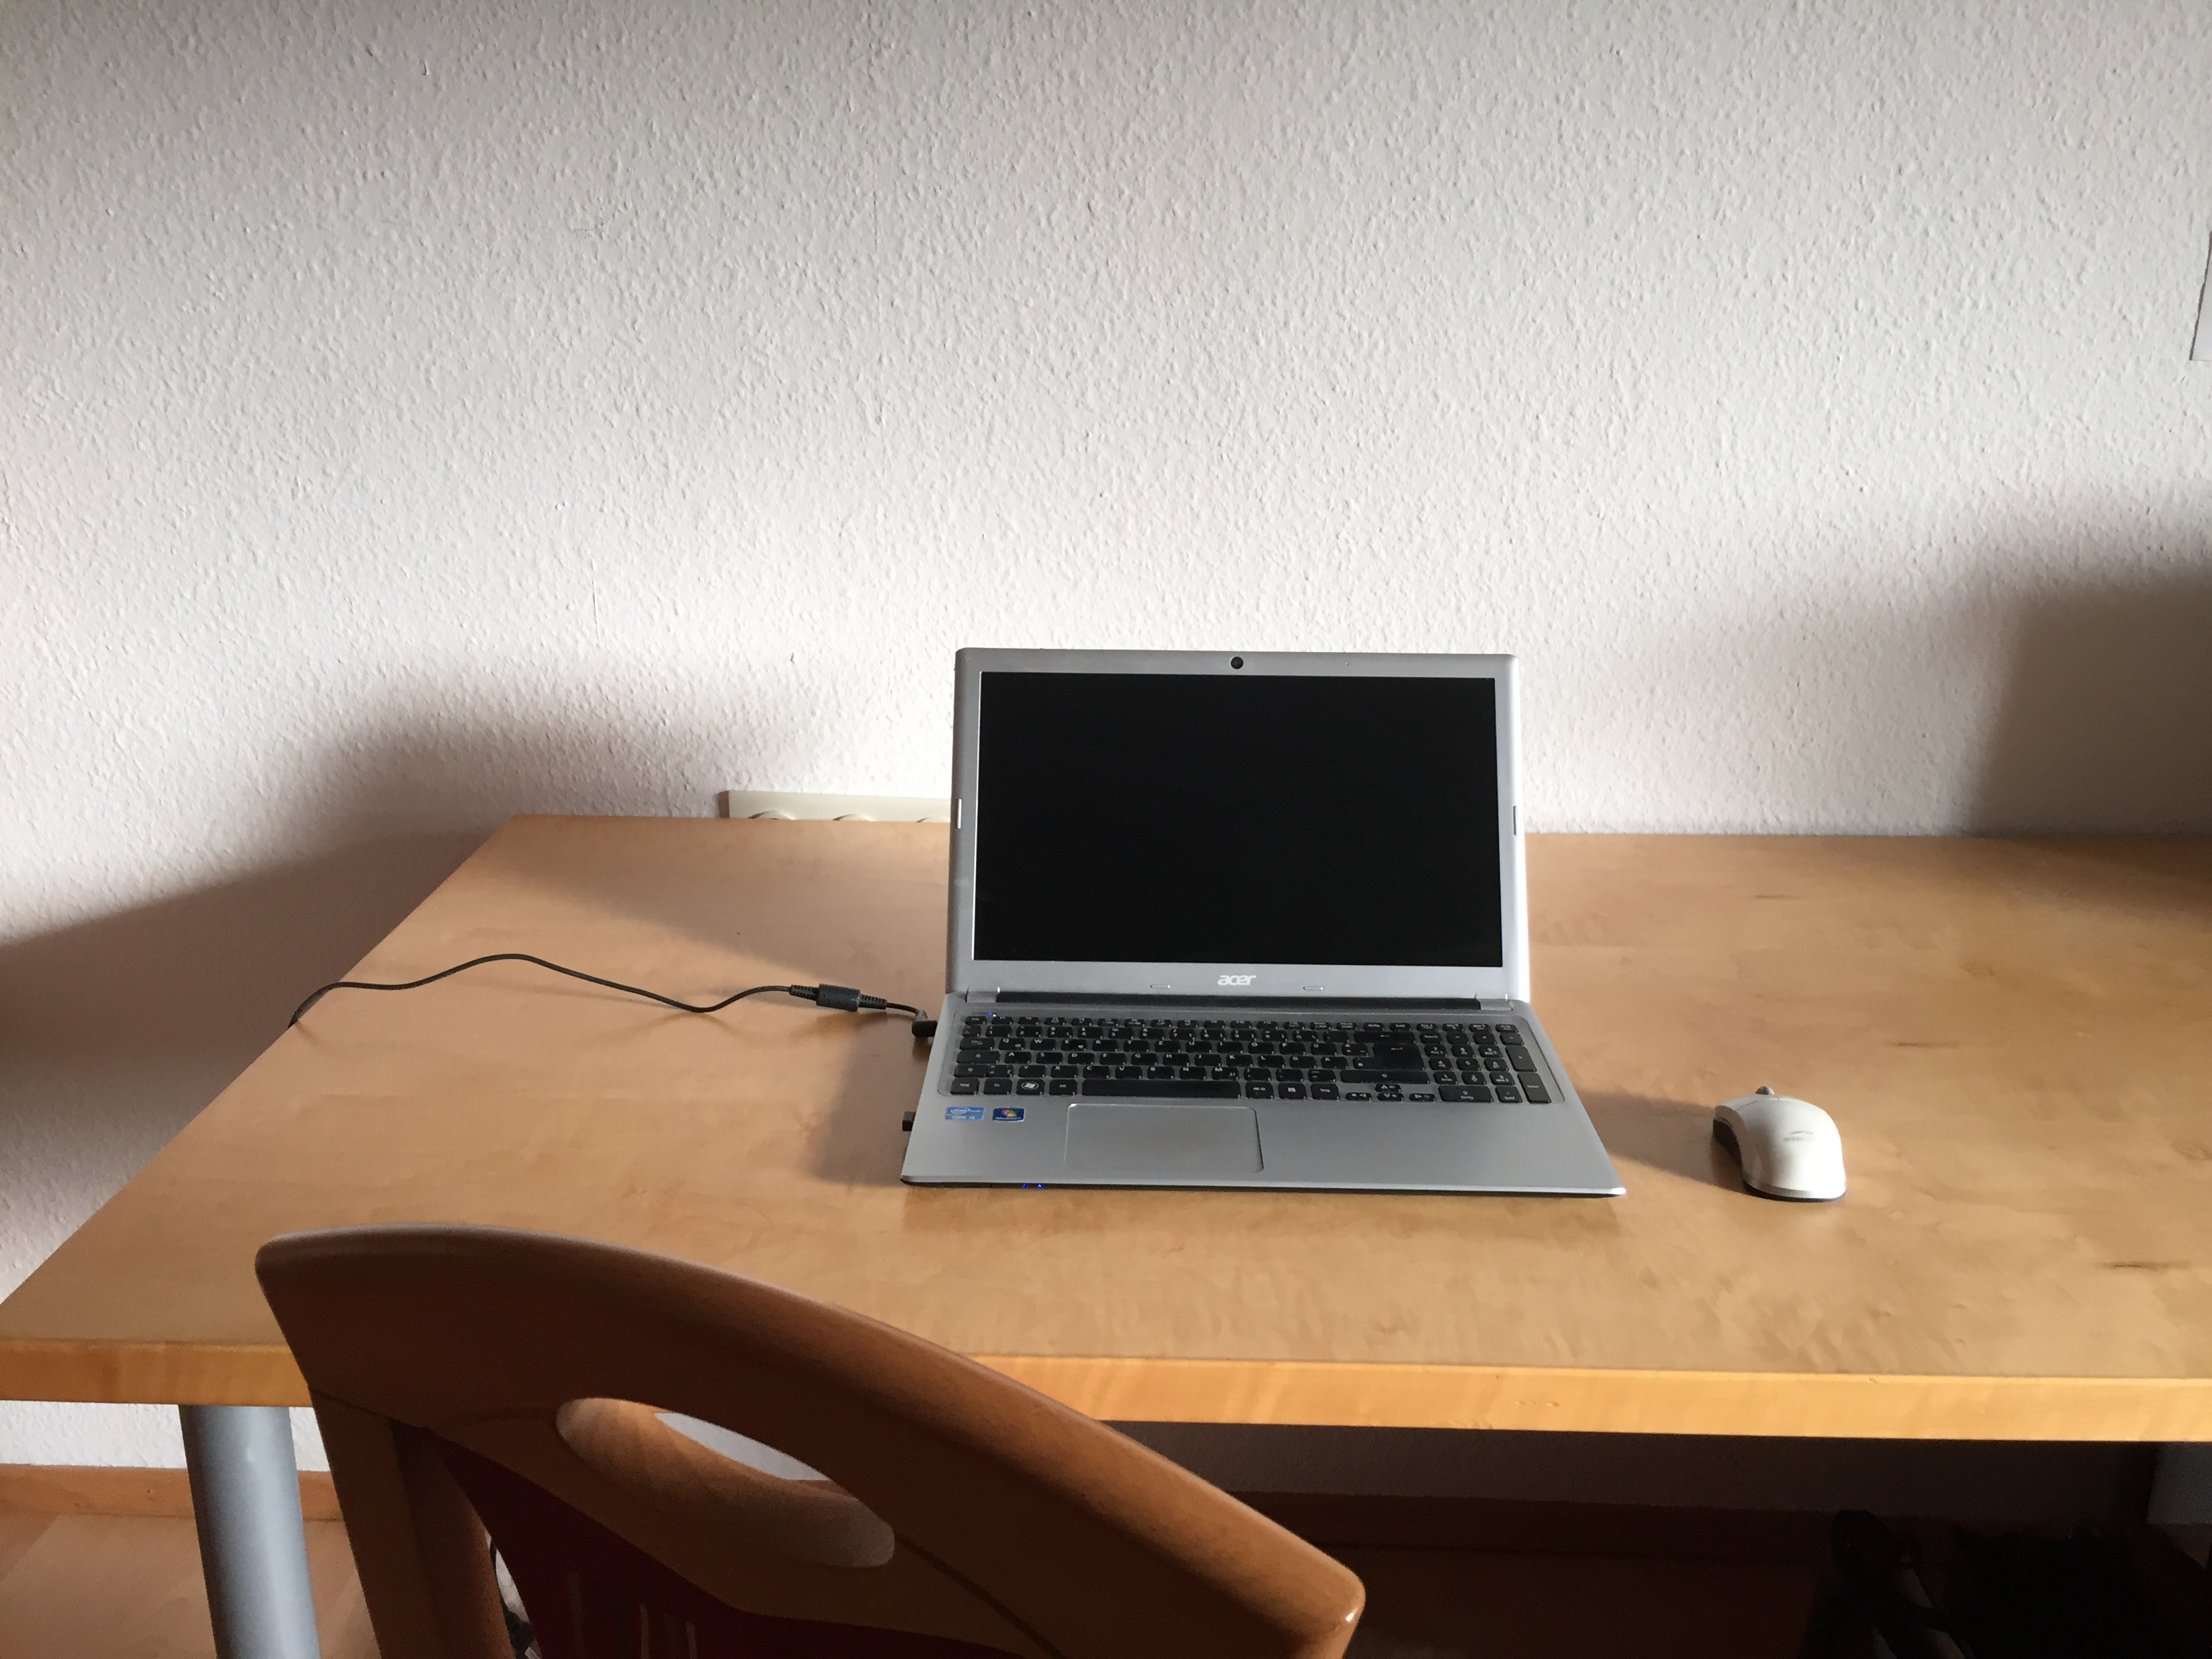
\includegraphics[width=.45\linewidth]{study1/setup_d.JPG}}\hfill
\subfloat[The hardware for the installation set up in the other room \label{fig:setup_1}]
  {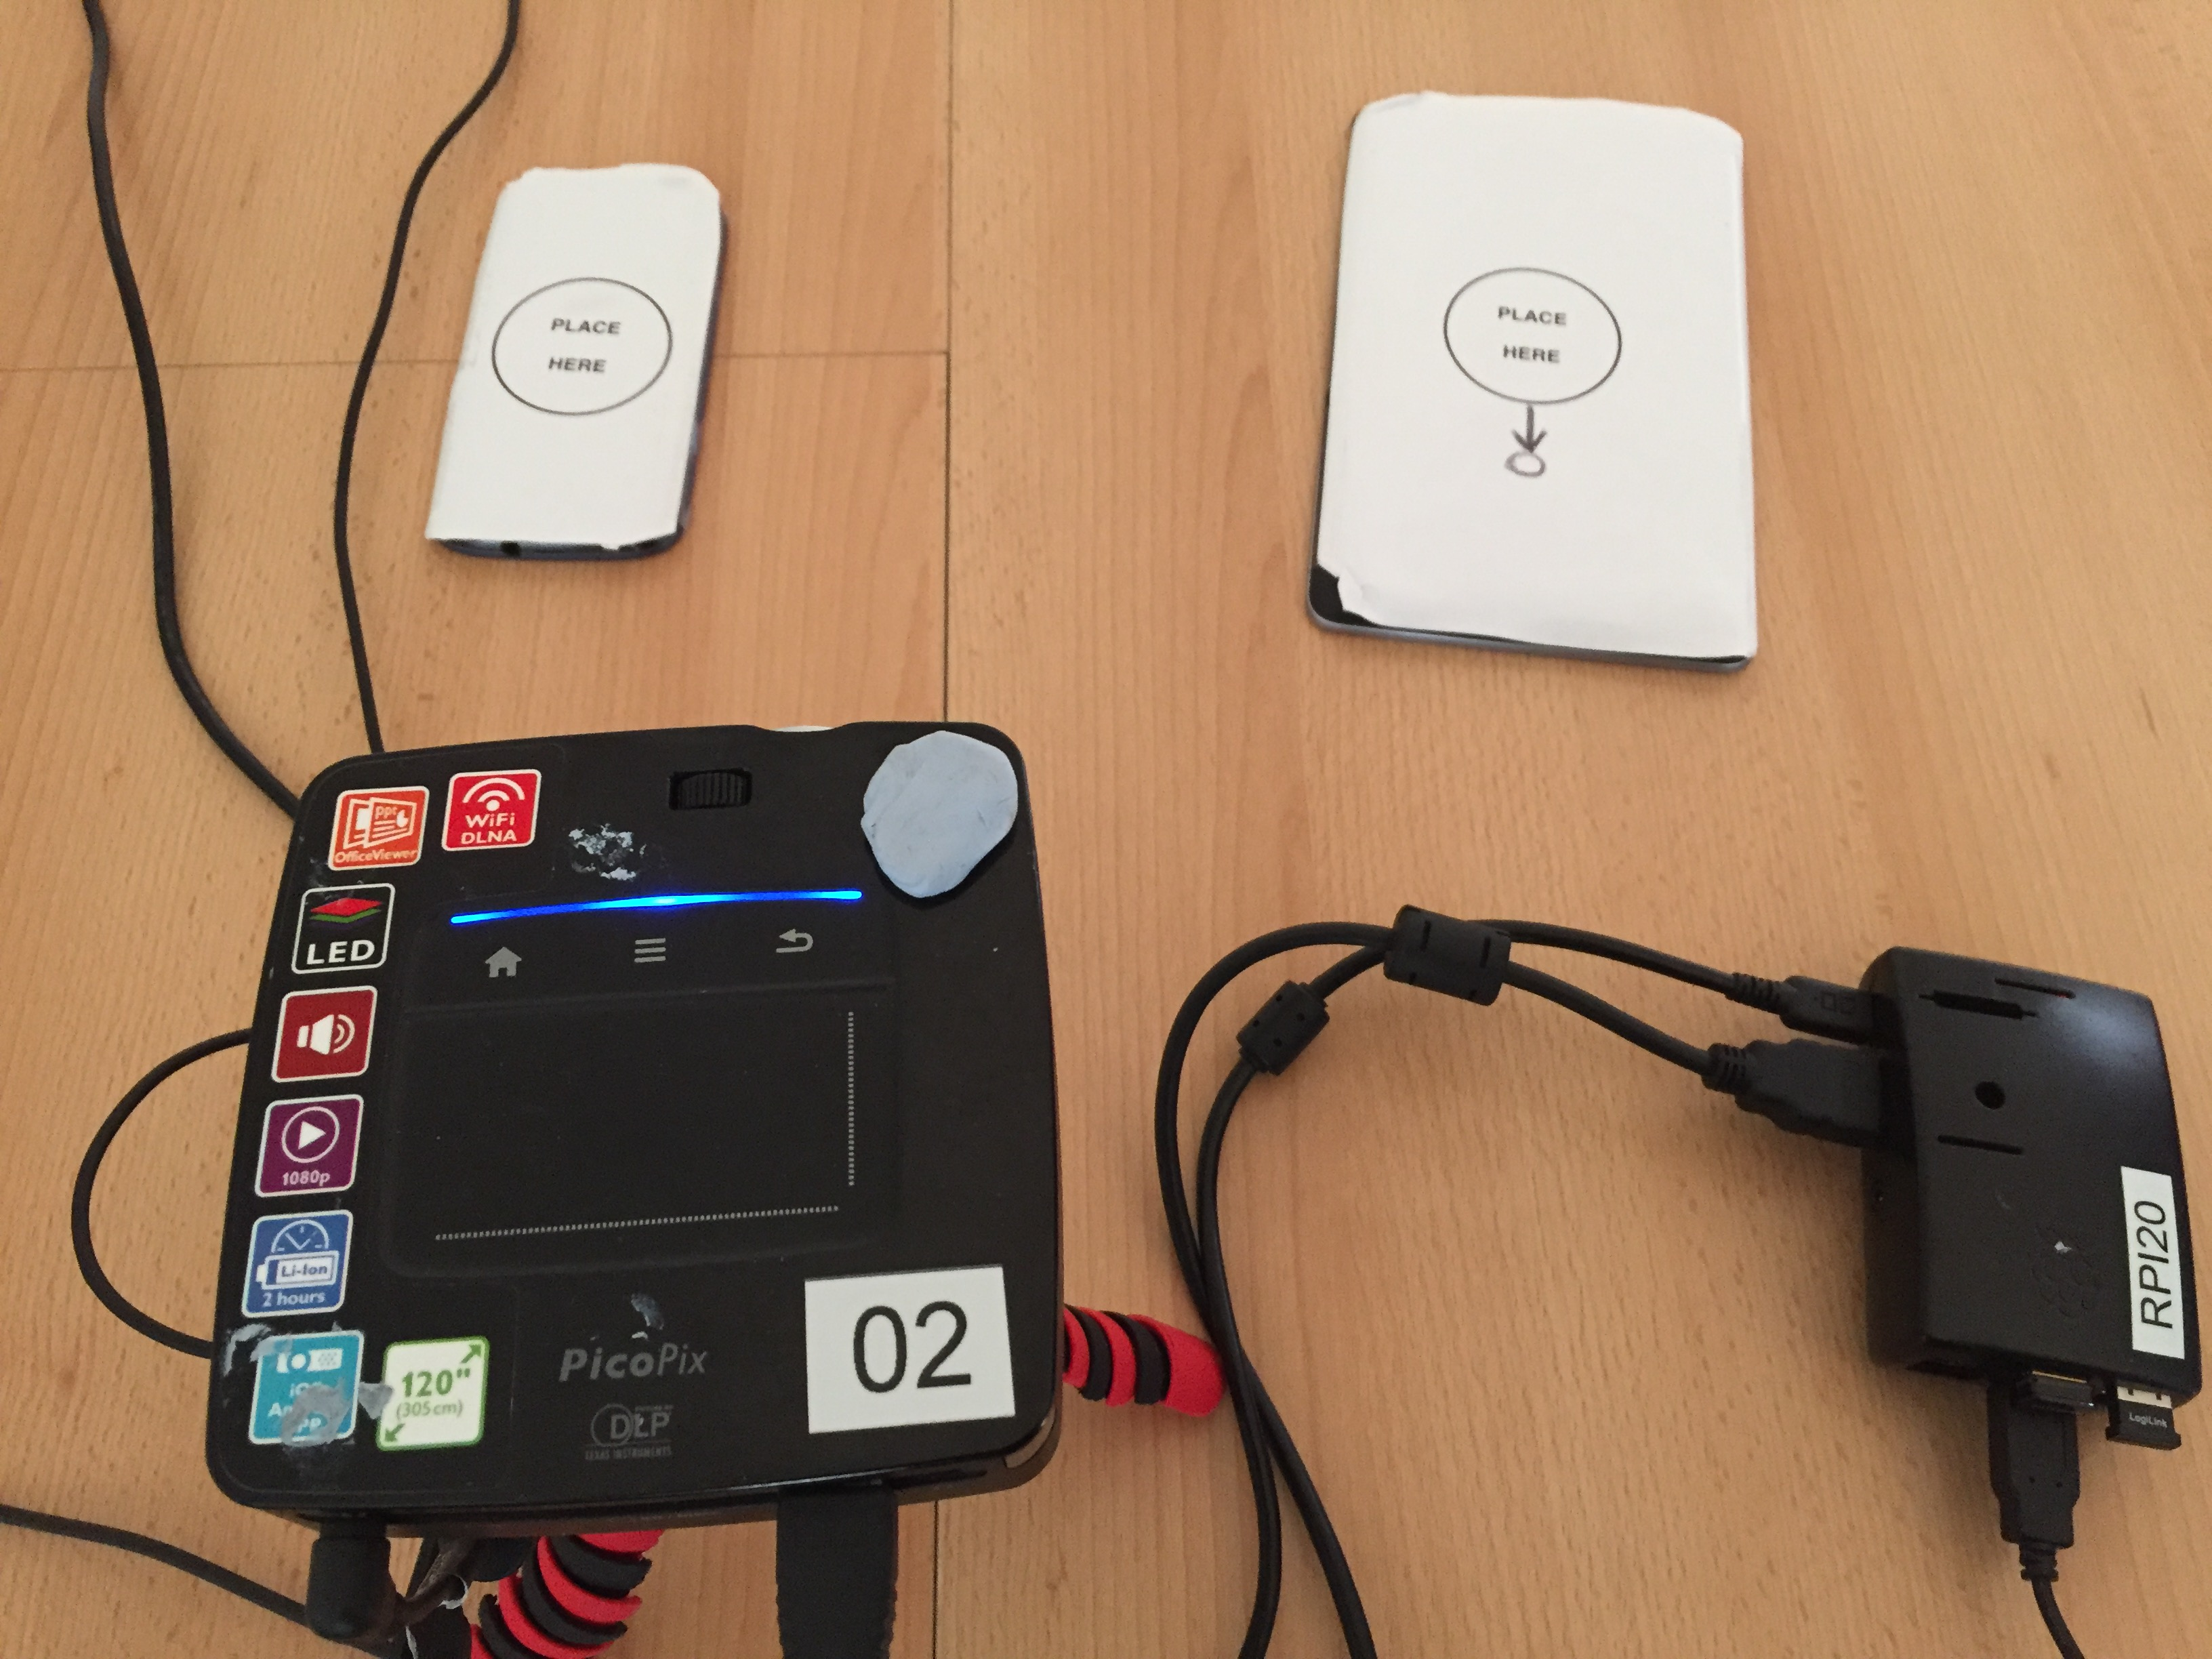
\includegraphics[width=.45\linewidth]{study1/setup_1.JPG}}\hfill
\caption{The general setup of the pre-study}
\end{figure}

For the study 9 participants (3 female, 6 male) with an average age of 25 years and a different level of technical expertise (from "I know how to code" to "I only use my computer to browse the internet") where recruited. The participants where not required to have any technical expertise and were selected randomly. Four of them used software like Adobe Photoshop and Microsoft Powerpoint quite often, the others did not hear of it or only used it once. Two of the participants were also familiar with the content management system Wordpress. The participants did not get any reward for participating at the study.

The test-environment was set up in two different rooms. In the first room there was a desktop computer where the participants had to create the content which they wanted to display in their installation as well as the rules which would provide the interactivity. Therefore, a server instance of the meSchup platform was running on the desktop computer. In the second room there was set up a RaspberryPi connected to a projector serving as the displaying device and two Android devices which were used as NFC-Readers. All devices were connected to the local network. Before the participants started testing the Android devices were configured as NFC-Readers in the meSchup platform and one template which provided the needed behavior functionality to solve the given tasks was implemented. The reason for this was the assumption that non-professionals will also use rule templates for creating interactivity and will not program the code on their own.

\subsection{Procedure and Tasks}
Every participant got a short introduction to the test environment but not to the VEII toolkit. They all had to accomplish the same task: Create an interactive installation using the toolkit which provides multiple slides featuring different content and which uses NFC-Tags registering on a NFC-Reader to switch between them. This task was divided into the following steps:

\textbf{Step 1: Content creation}
\newline
The participant should create two slides with different content on the desktop computer.

\textbf{Step 2: Creating interactivity} 
\newline
The participant should use a template to create rules which provide the NFC functionality.

\textbf{Step 3: Deploy content} 
\newline
The participant should deploy the created content on the display device in the second room 

\textbf{Step 4: Adapt content on-site} 
\newline
The participant should visit the installation with a mobile device and adapt to content according to the environment.

\textbf{Step 5. Switch to deployment mode:} 
\newline
The participant should use the mobile device two switch the installation from the "Live-Edit" mode to the "Deployment" mode.

\textbf{Step 6: Test the interactivity} 
\newline
The participant should use a NFC tag on the different NFC-Reader two switch between the created slides.

The participants were allowed to ask questions during the whole process, most of them did not need to make use of this possibility. After finishing the task, every participant had to answer a System Usability Scale (SUS) questionnaire with 10 questions. Afterwards each participant took place in a semi-structured interview which lasted about 15 minutes. The questionnaire and the questions of the interview are shown in Appendix\ref{prestudy}. On average, the total duration of a study per participant lasted 45 minutes.

\subsection{Study results and discussion}
In this section the observations about participants' creation strategies as well as the results of the System Usability Scale (SUS) questionnaire, the participants qualitative feedback and consequences derived from these insights are discussed.
%The goal of the pre study was to test usability of the toolkit with non-professionals with focus on the qualitative feedback of the participants afterwards. Therefore, we used the System Usability Scale (SUS) and an interview afterwards to evaluate the participant experiences. 
\subsubsection{Creation strategies}

\begin{figure}
\subfloat[A participant creating content on a desktop computer.\label{fig:study1user}]
  {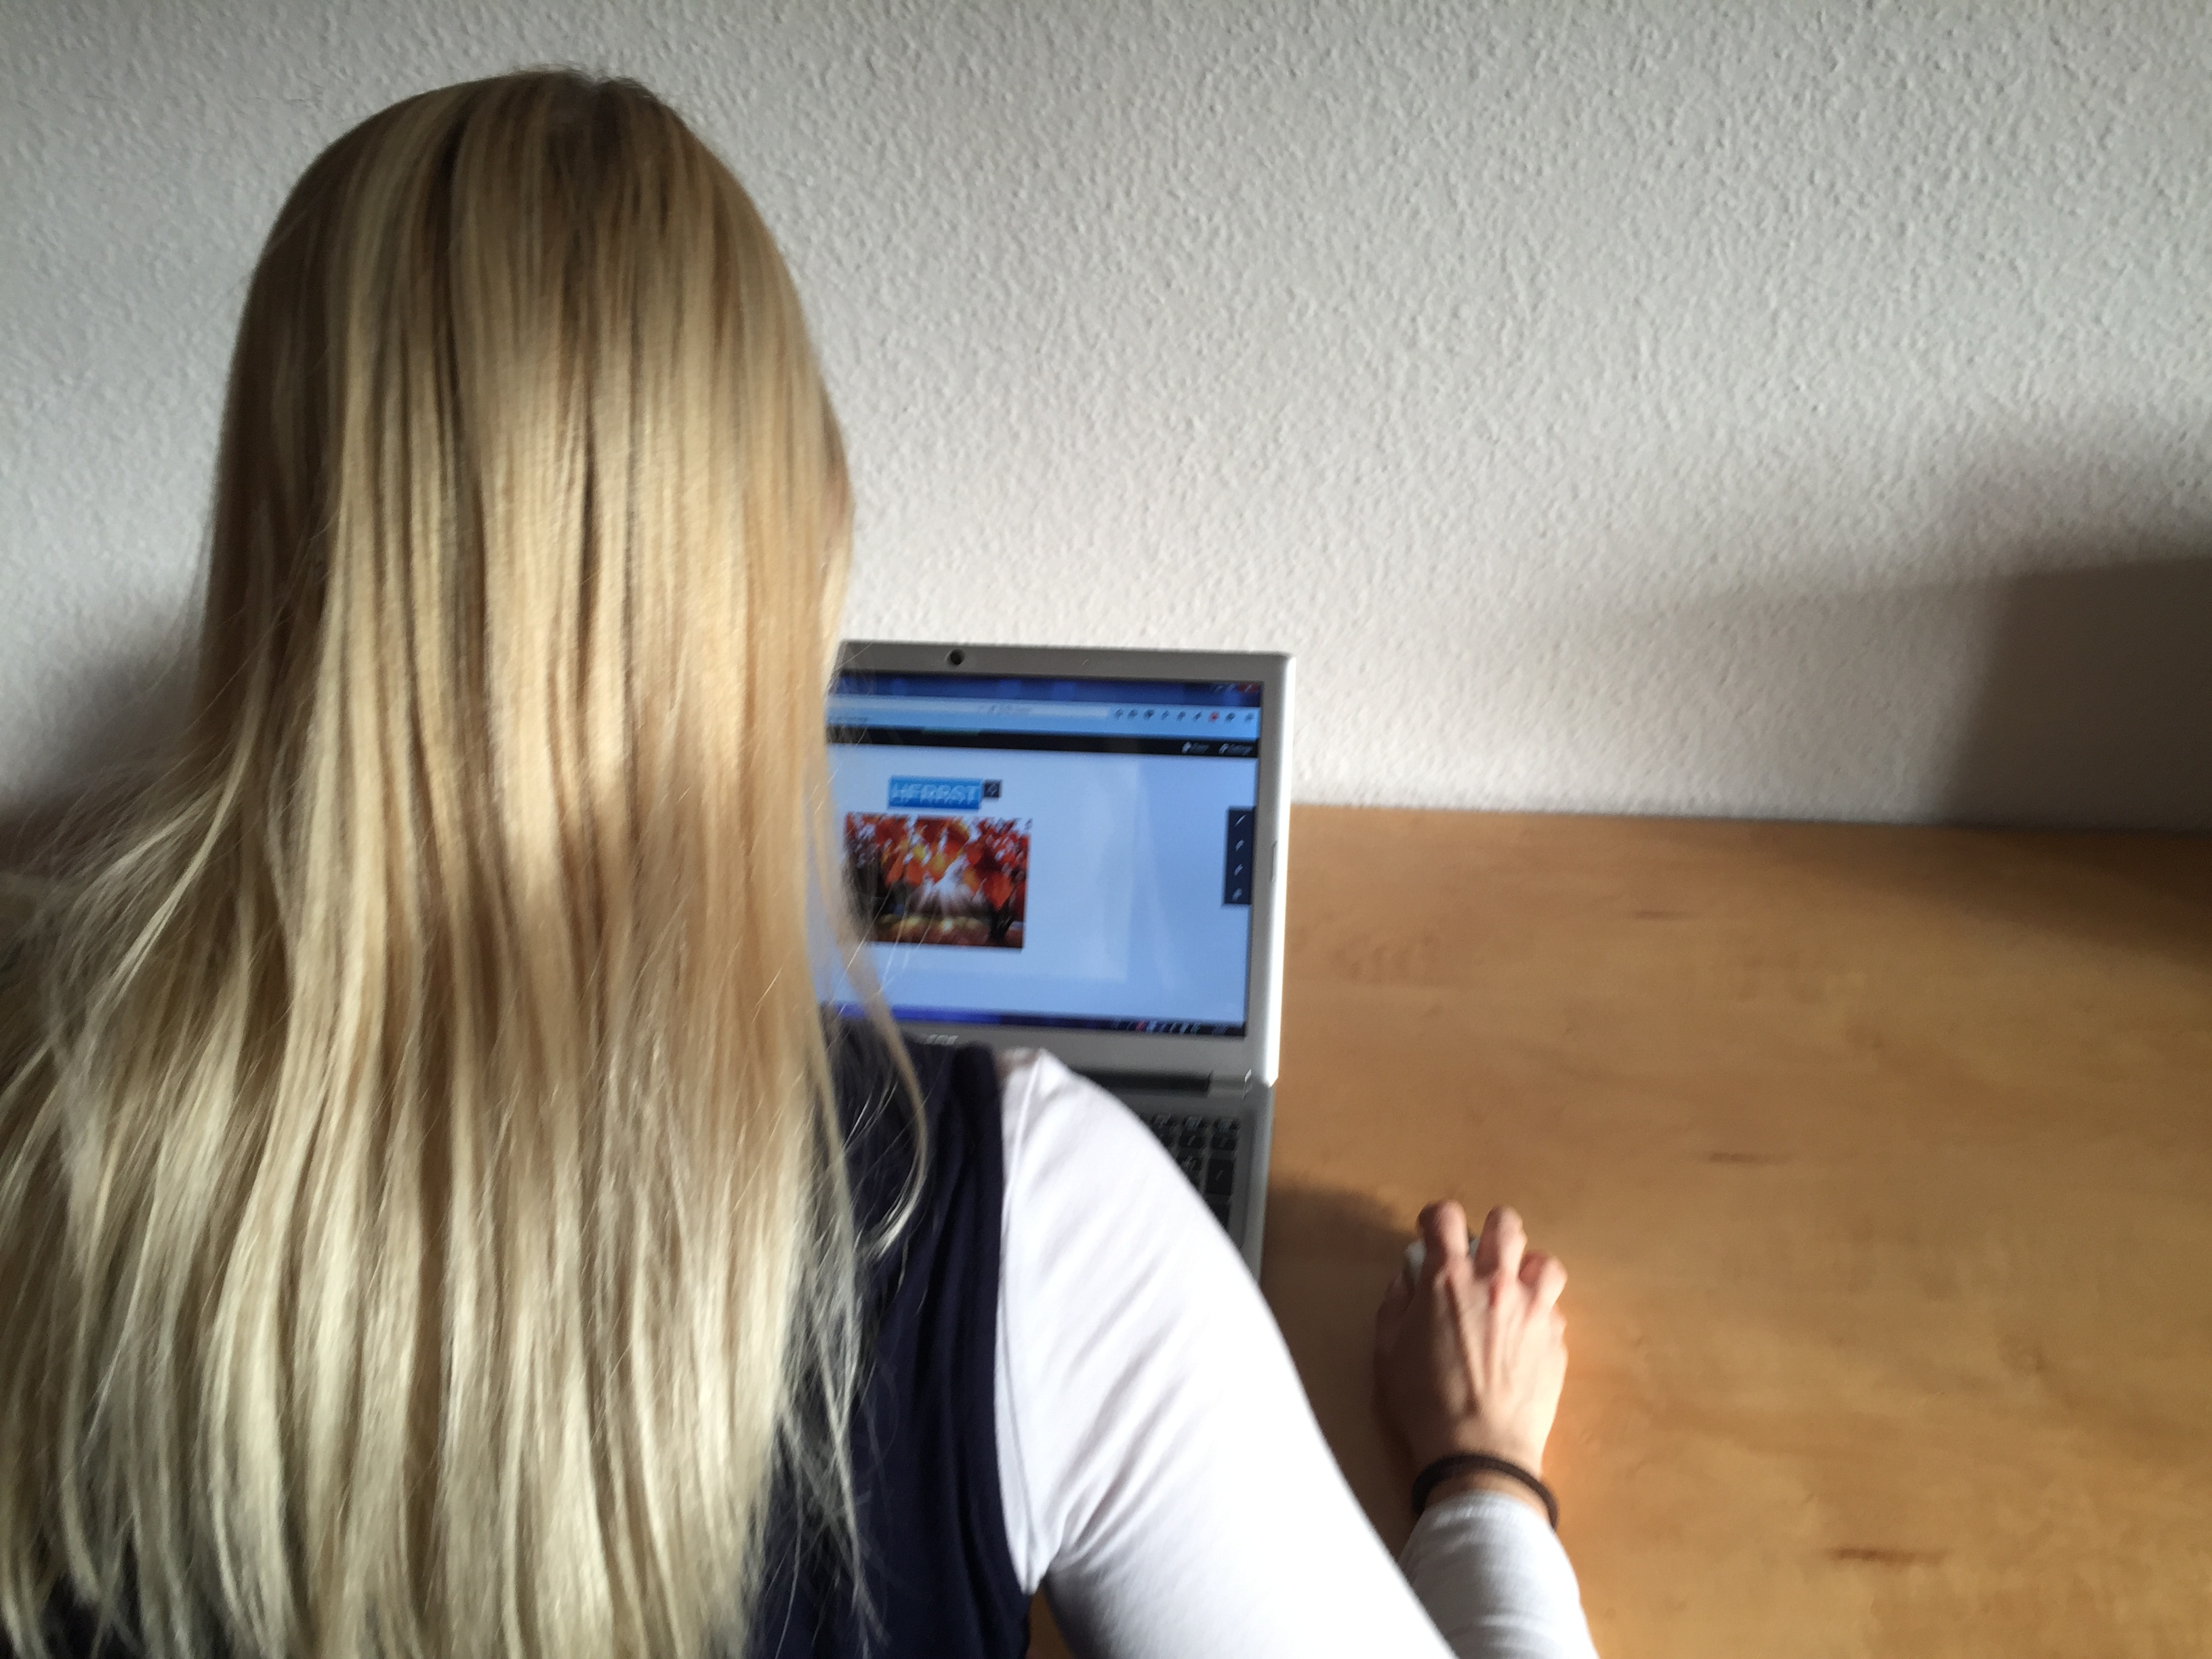
\includegraphics[width=.45\linewidth]{study1/p_desktop.JPG}}\hfill
\subfloat[A participant using a mobile device to tweak content on-site\label{fig:study2user}]
  {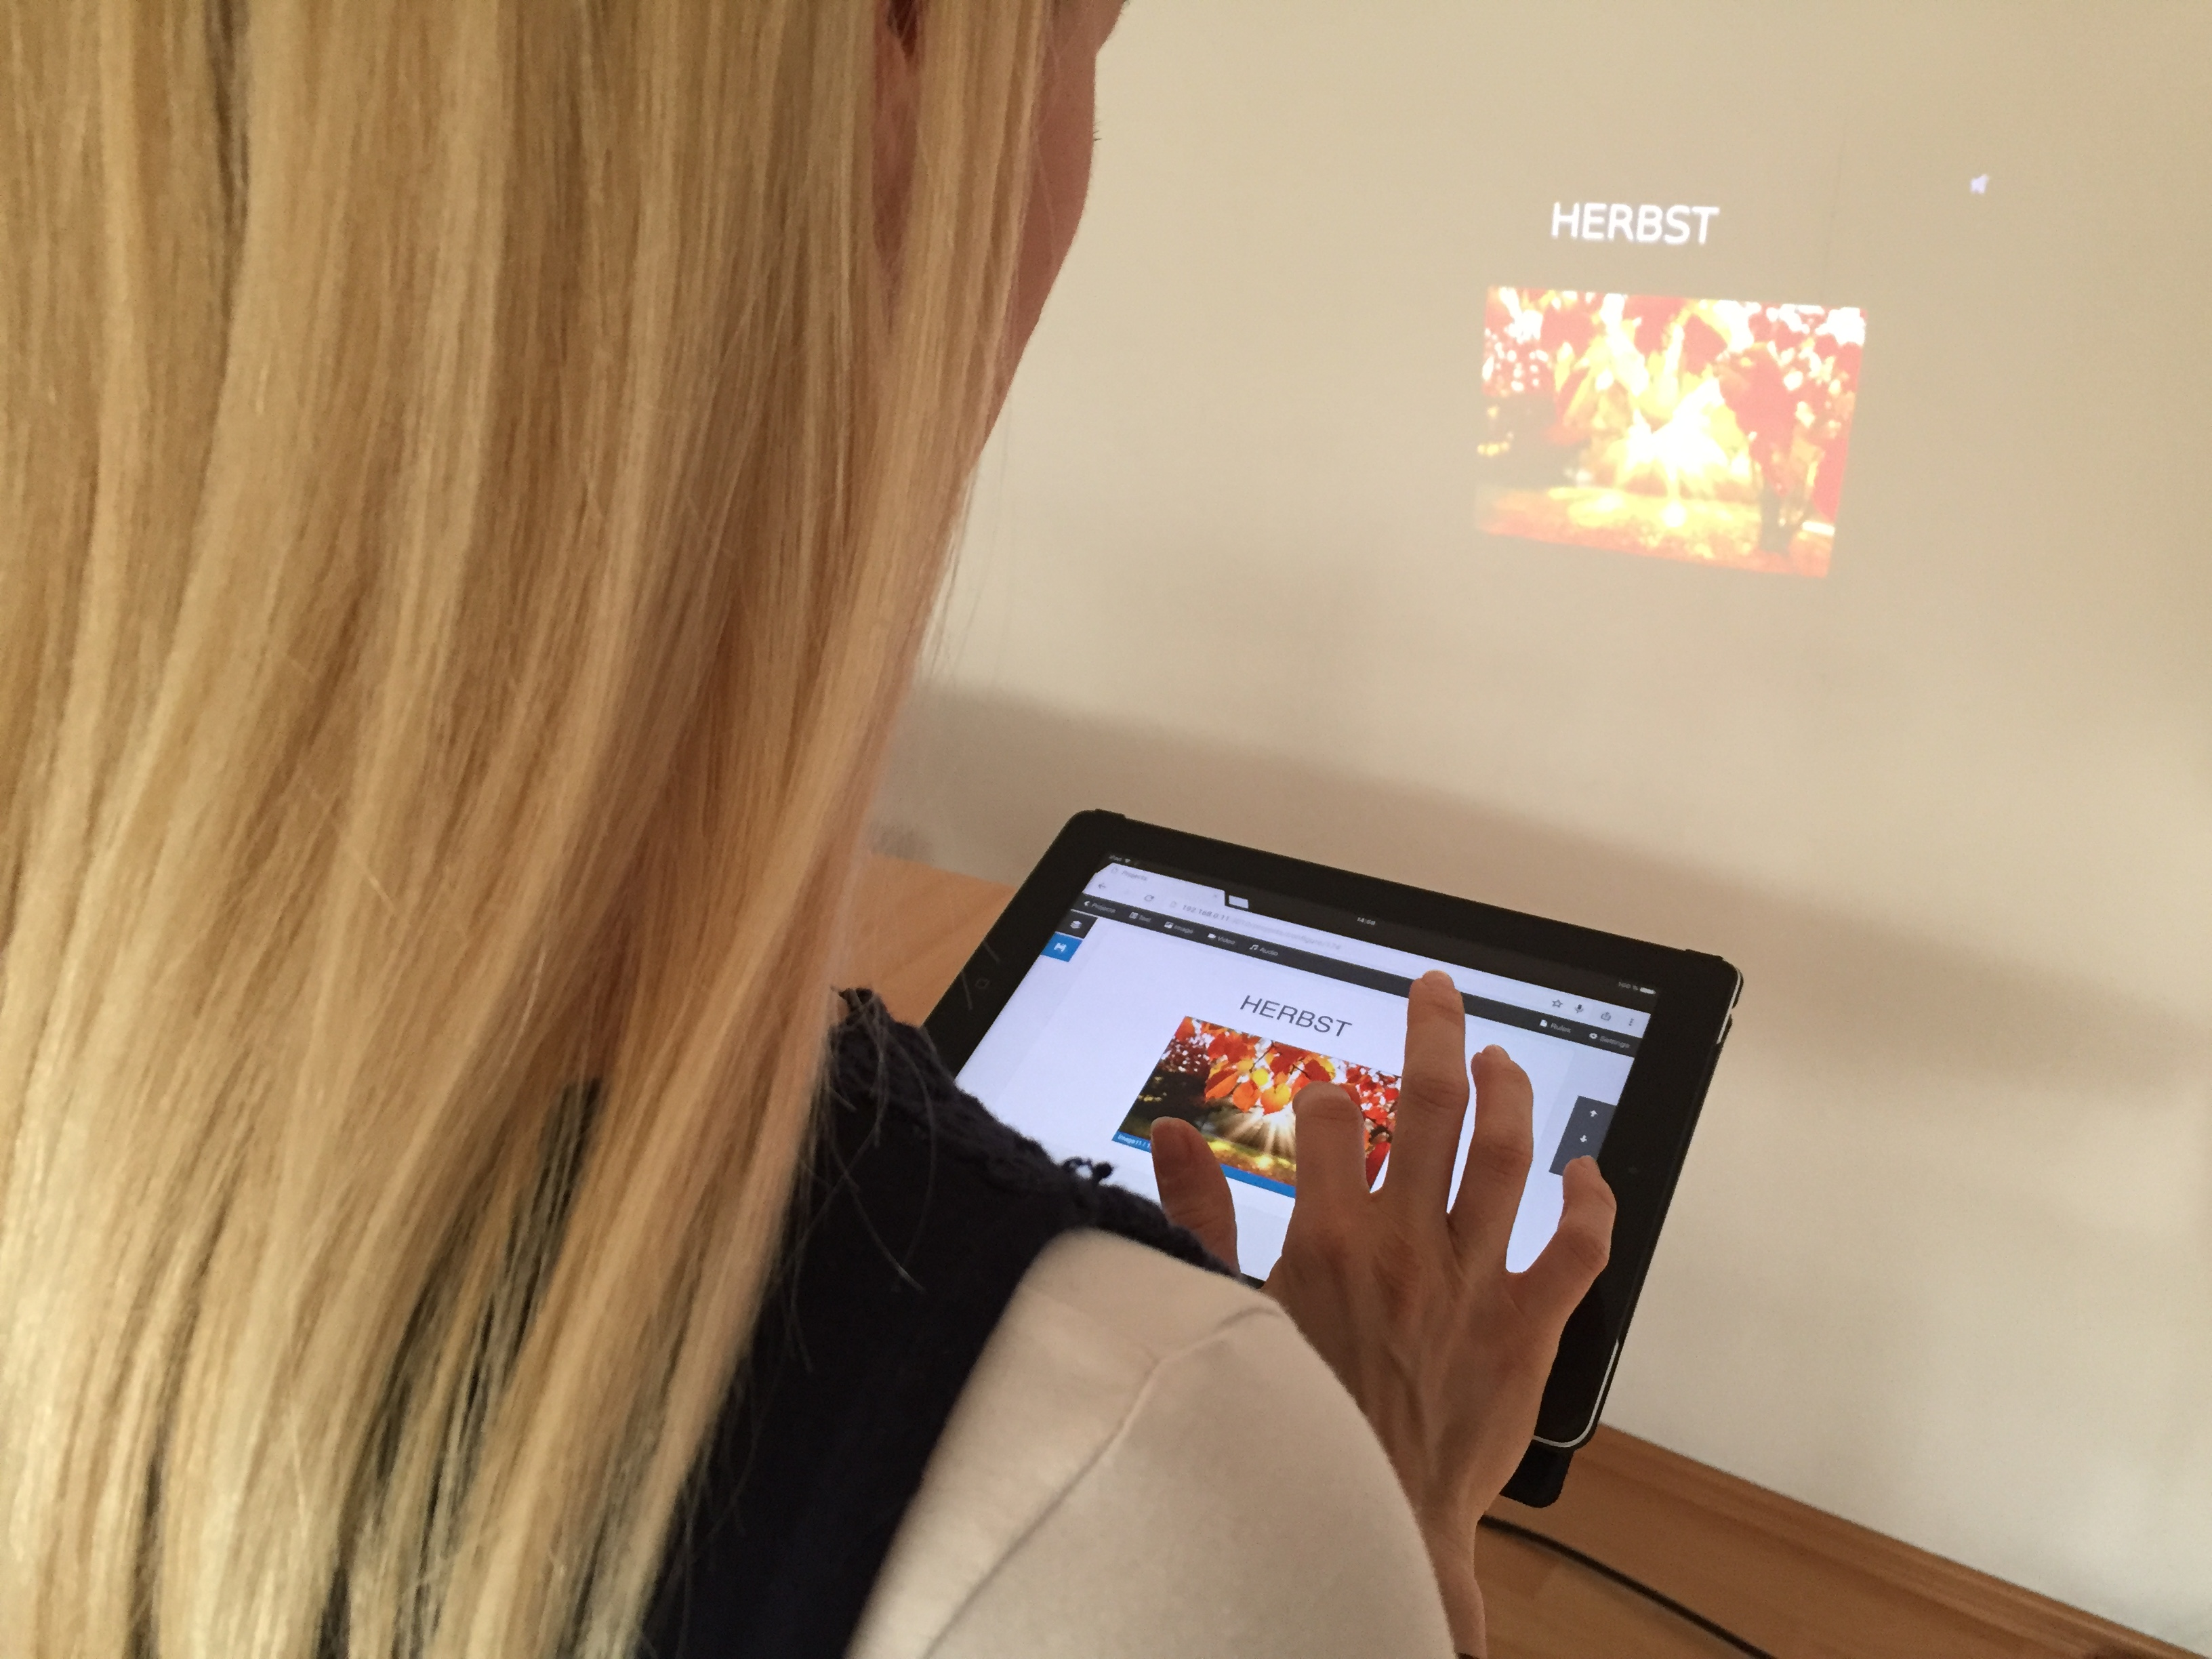
\includegraphics[width=.45\linewidth]{study1/p_onsite.JPG}}\hfill
\caption{A participant during the pre-study}
\end{figure}

All participants successfully created, adapted and tested an interactive installation with digital content and therefore fulfilled the given task in the study. The average time of completing the task was 28 minutes. One  observation was that the participants had a similar creation strategy: after about 30 seconds of just viewing at the user interface to get a general overview, most of the participants started by trying out all different UI buttons to see what happens. Afterwards they started adding and adapting content, mostly more than needed. Some of them got so engrossed in optimizing their content and using the various transform options that they forgot to go on with the next step of the task: P6 said, \textit{"I really liked the possibility to adapt the content as I needed it like rotating and scaling images without the need of using external programs"}. Then the participants switched to the Rule Editor where they created two behavior rules by using templates. P4 noted: \textit{"It was great that I did not have to program the rules on my own. Through the description I knew which template to use"}. The participants where surprised how simple it is to provide interactivity and make use of complex hardware. P1 commented: \textit{"I created something with technology I didn't even heard about within 20 minutes"}. Every participant created a rule and configured it within no time. Last the participants went to the installation and adapted the content on-site where all participants used the mobile device to adapt the content in the target environment. 

\subsubsection{Working with the system}
The participants were very positive about working with the VEII toolkit. They found it intuitive and easy to learn which is confirmed by the average score of 3.7 (SD = 0.63, 0.0 - lowest, 4.0 - highest) of the question "I would imagine that most people would learn to use this system very quickly" of the SUS. Every participant learned to use the system within 10 minutes without the need of any assistance. Nevertheless, the participants also mentioned aspects of the system which should be improved. This is shown by the score of 2.8 (SD = 0.75) in the SUS of the question "I thought there was too much inconsistency in this system". In this case most participants were confused about the placing or the meaning of specific UI elements. For example there was a "Done"- and a "Close"-Button in the rule creation view which often got mixed up. The VEII toolkit ended up with a total score of 82.5 in the SUS. As visible in Figure~\ref{fig:prestudyresult1}, every question got a score above the standard average score of 68 which is the threshold of a usable system. Any software with a lower score as 68 is considered to be not usable.
\newline

\begin{figure}
  \begin{center}
    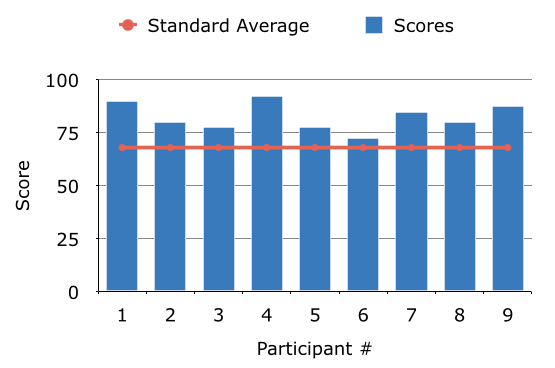
\includegraphics[width=.8\textwidth]{study1.png}
    \caption{The results of the pre-study SUS questionnaire by participants}
    \label{fig:prestudyresult1}
  \end{center}
\end{figure}

\textbf{Working with the VEII Slide Editor}
\newline
The participants thought the Slide Editor is intuitive and easy to use which is based on structural similarities to existing software. P4 said, \textit{"The structure of the editor remembered me of Powerpoint which definitely helped me understand it more quickly"}. P2 commented: \textit{"The image management view felt like using Wordpress, which I often use"}. But also participants who did not have any technical background or knowledge of existing software got used to the VEII Slide Editor fast. P1 mentioned: \textit{"It is very convenient that I can compose the desired content by only using the mouse. If something did not fit, I could easily modify it"}. Furthermore, the participants were convinced of the variety of transform options of content like scale, moving and rotating which were available within the VEII Slide Editor. P6 said, \textit{"Adapting the position or the size of content is very easy. I really liked that I could adapt content on the mobile device as easy as on the desktop computer"}.
\newline

\textbf{Working with the VEII Rule Editor}
\newline
First the participants needed to create a behavior rule by choosing a template and defining a name and an optional description. In this case the UI seemed to be confusing. P4 mentioned: \textit{"Firstly I was not sure if I need to set a name and description for the chosen template or if I would create a new one with it"}.
Nevertheless, all participants were convinced of the story-approach especially because the complex code was hidden. P9 said, \textit{"Through the story I knew what to do but I did not have to know how it technically works"}. P8 confirmed: \textit{"I read the text so I could choose accordingly. Code would be confusing"}. Furthermore, the participants liked that they could configure the rule by using simple UI elements like select boxes. \textit{"I found it easy to select from the drop down, which NFC-Reader I want to use. It was very clear"} added P3. Some of the participants found that the labels of the UI elements within the story were unnecessary. P2 said, \textit{"I was a bit confused of some of the labels within the story, they sounded very technical, but at least I realized that I do not need them"}. In this part the two buttons "Done" and "Save" often got mixed up. Some participants pressed the "Done"-Button after configuring the rule and wondered why nothing changed. All in all the participants described working with the system as \textit{"simple and clear"} (P8).
\newline

\textbf{On-site editing}
\newline
All participants found that the on-site editing approach is very convenient and easy. Almost everyone said that he had particularly liked that part. P5 noted: \textit{"One can see how it looks finished and then easily customize it"}. P8 said, \textit{"I liked the combination of preparation and alignment in the live-edit mode. I could easily modify my content without big effort"}. P1 and P5 mentioned that using a mobile device this way was very new for them but they were excited about the immediate feedback. 
Not every participant tested the correction of distortion by tilting the mobile device because it was not part of the task. But those who tried this option were very enthusiastic about it. P6 said, \textit{"This was something special that I did not know before. It would be great to correct the content if the projector is not positioned even to the wall"}. Furthermore, the participants were convinced about separating the content creation and adaptation from presenting content and triggering behavior rules by using two different modes.
\newline

\subsubsection{Feedback}
However, the participants in general desired more feedback from the system. Because of missing feedback or explanation of UI elements some participants did get stuck for a few minutes. P6 noted: \textit{"Sometimes it was not entirely clear on what button I have to click next"}. The participants proposed to realize feedback in the form of tooltips to get further information about UI elements. P3 said, \textit{"It would be great if the symbols would be explained if I position the mouse over them"}. P4 and P6 had some problems with the structure of the menu within the rule creation views. P4 mentioned: \textit{"The menu was a bit difficult to use, sometimes the button I needed was not where it used to be in similar software"}. In this case P4 meant the "Save"-Button of the rule which was placed in the upper right corner and he expected it to be in the lower right corner where the "Done"-Button was placed. P1, P3, P4, P6 and P9 also mentioned that they would like to have a short introduction to the system in form of a guided tour which introduces the most important features as well as a short tutorial or example video of how to create an interactive installation. P9 said, \textit{"A short tour at the beginning which highlights the most important features and explains them would make it easier to start with the system"}. P3 added: \textit{"In some software I was using, there were short introduction videos to show the user what to do, I could imagine using an introduction video for this software as well"}.
 
The participants also mentioned different areas where they could imagine using this system. Some of them had more basic ideas like P2, P3 and P6 mainly mentioned all kinds of public display in cities, at train and bus stations as well as at the airport. Especially the participants wished to get further information while interacting with the public display. For example they want to use their digital ticket at the airport to get direction instruction to find their terminal just by getting close to the display. Another example was to get more information about the punctuality of the train they want to take by using their online ticket. P1 and P5 where looking beyond the box and thought about supermarkets and car dealers where it is currently not common practice to use interactive displays. P5 said, \textit{"I could imagine car dealers to give visitors car keys which have some kind of sensor attached or integrated. This would enable visitors to get further information at specific places in the store"}. P1 added: \textit{"If there would be displays in supermarkets I could use them to get more information about the products"}. In this case P1 did not think about which sensors to use but it is conceivable that manufacturers could integrate for example NFC-Technology within their packing of products. P7 is professionally often at fairs and sometimes he has to set up exhibitions stands for his company as well. P7 noted: \textit{"I really would like to use this system at one of our presentations at a fair. We would often like to change some small details but do not know how to change the content of the displays because external companies prepared them for us"}.

\subsubsection{Improvements}
Mostly the participants mentioned to improve the feedback of the system. The lack of information somehow resulted in participants misunderstanding the system and therefore they needed more time to solve the task. The Participants proposed multiple ways to improve the systems' feedback to the user. 

\begin{enumerate}
	\item{Integrating tooltips for UI elements}
	\item{Provide a guided tour at first usage}
	\item{Prepare tutorials or video-tutorials}
\end{enumerate}

Before doing the second study at Allard Pierson Museum in Amsterdam one of the proposed approaches was implemented. Using tooltips to give the user more information about specific UI elements seemed to be the most useful way to provide a permanent assistance while using the system. Furthermore, the other approaches could be implemented as well to provide further assistance to the user. Conceivable are not only tutorials for using the basic functionality of the system but also for implementing behavior rules using the story approach and the side panel with predefined sensor and actuator components as seen in Figure \ref{fig:ruleeditor}.

\section{Case Study II - Cultural Heritage}
The purpose of the study at Allard Pierson Museum in Amsterdam was to evaluate the VEII toolkit with Cultural Heritage Professionals in the context of a real exhibition space. One evaluation goal was to find out if the implemented approaches within the VEII toolkit are suitable for users who are not technical experts. Another goal was to collect the feedback of the CHPs and their suggestion on how the system can be improved and in what way they would integrate it in their professional environment. Therefore, a study with 5 participants was conducted performed over two days at Allard Pierson Museum in Amsterdam.

\subsection{Participants and Setup}

\begin{figure}
\subfloat[The participants desktop computer.\label{fig:setup}]
  {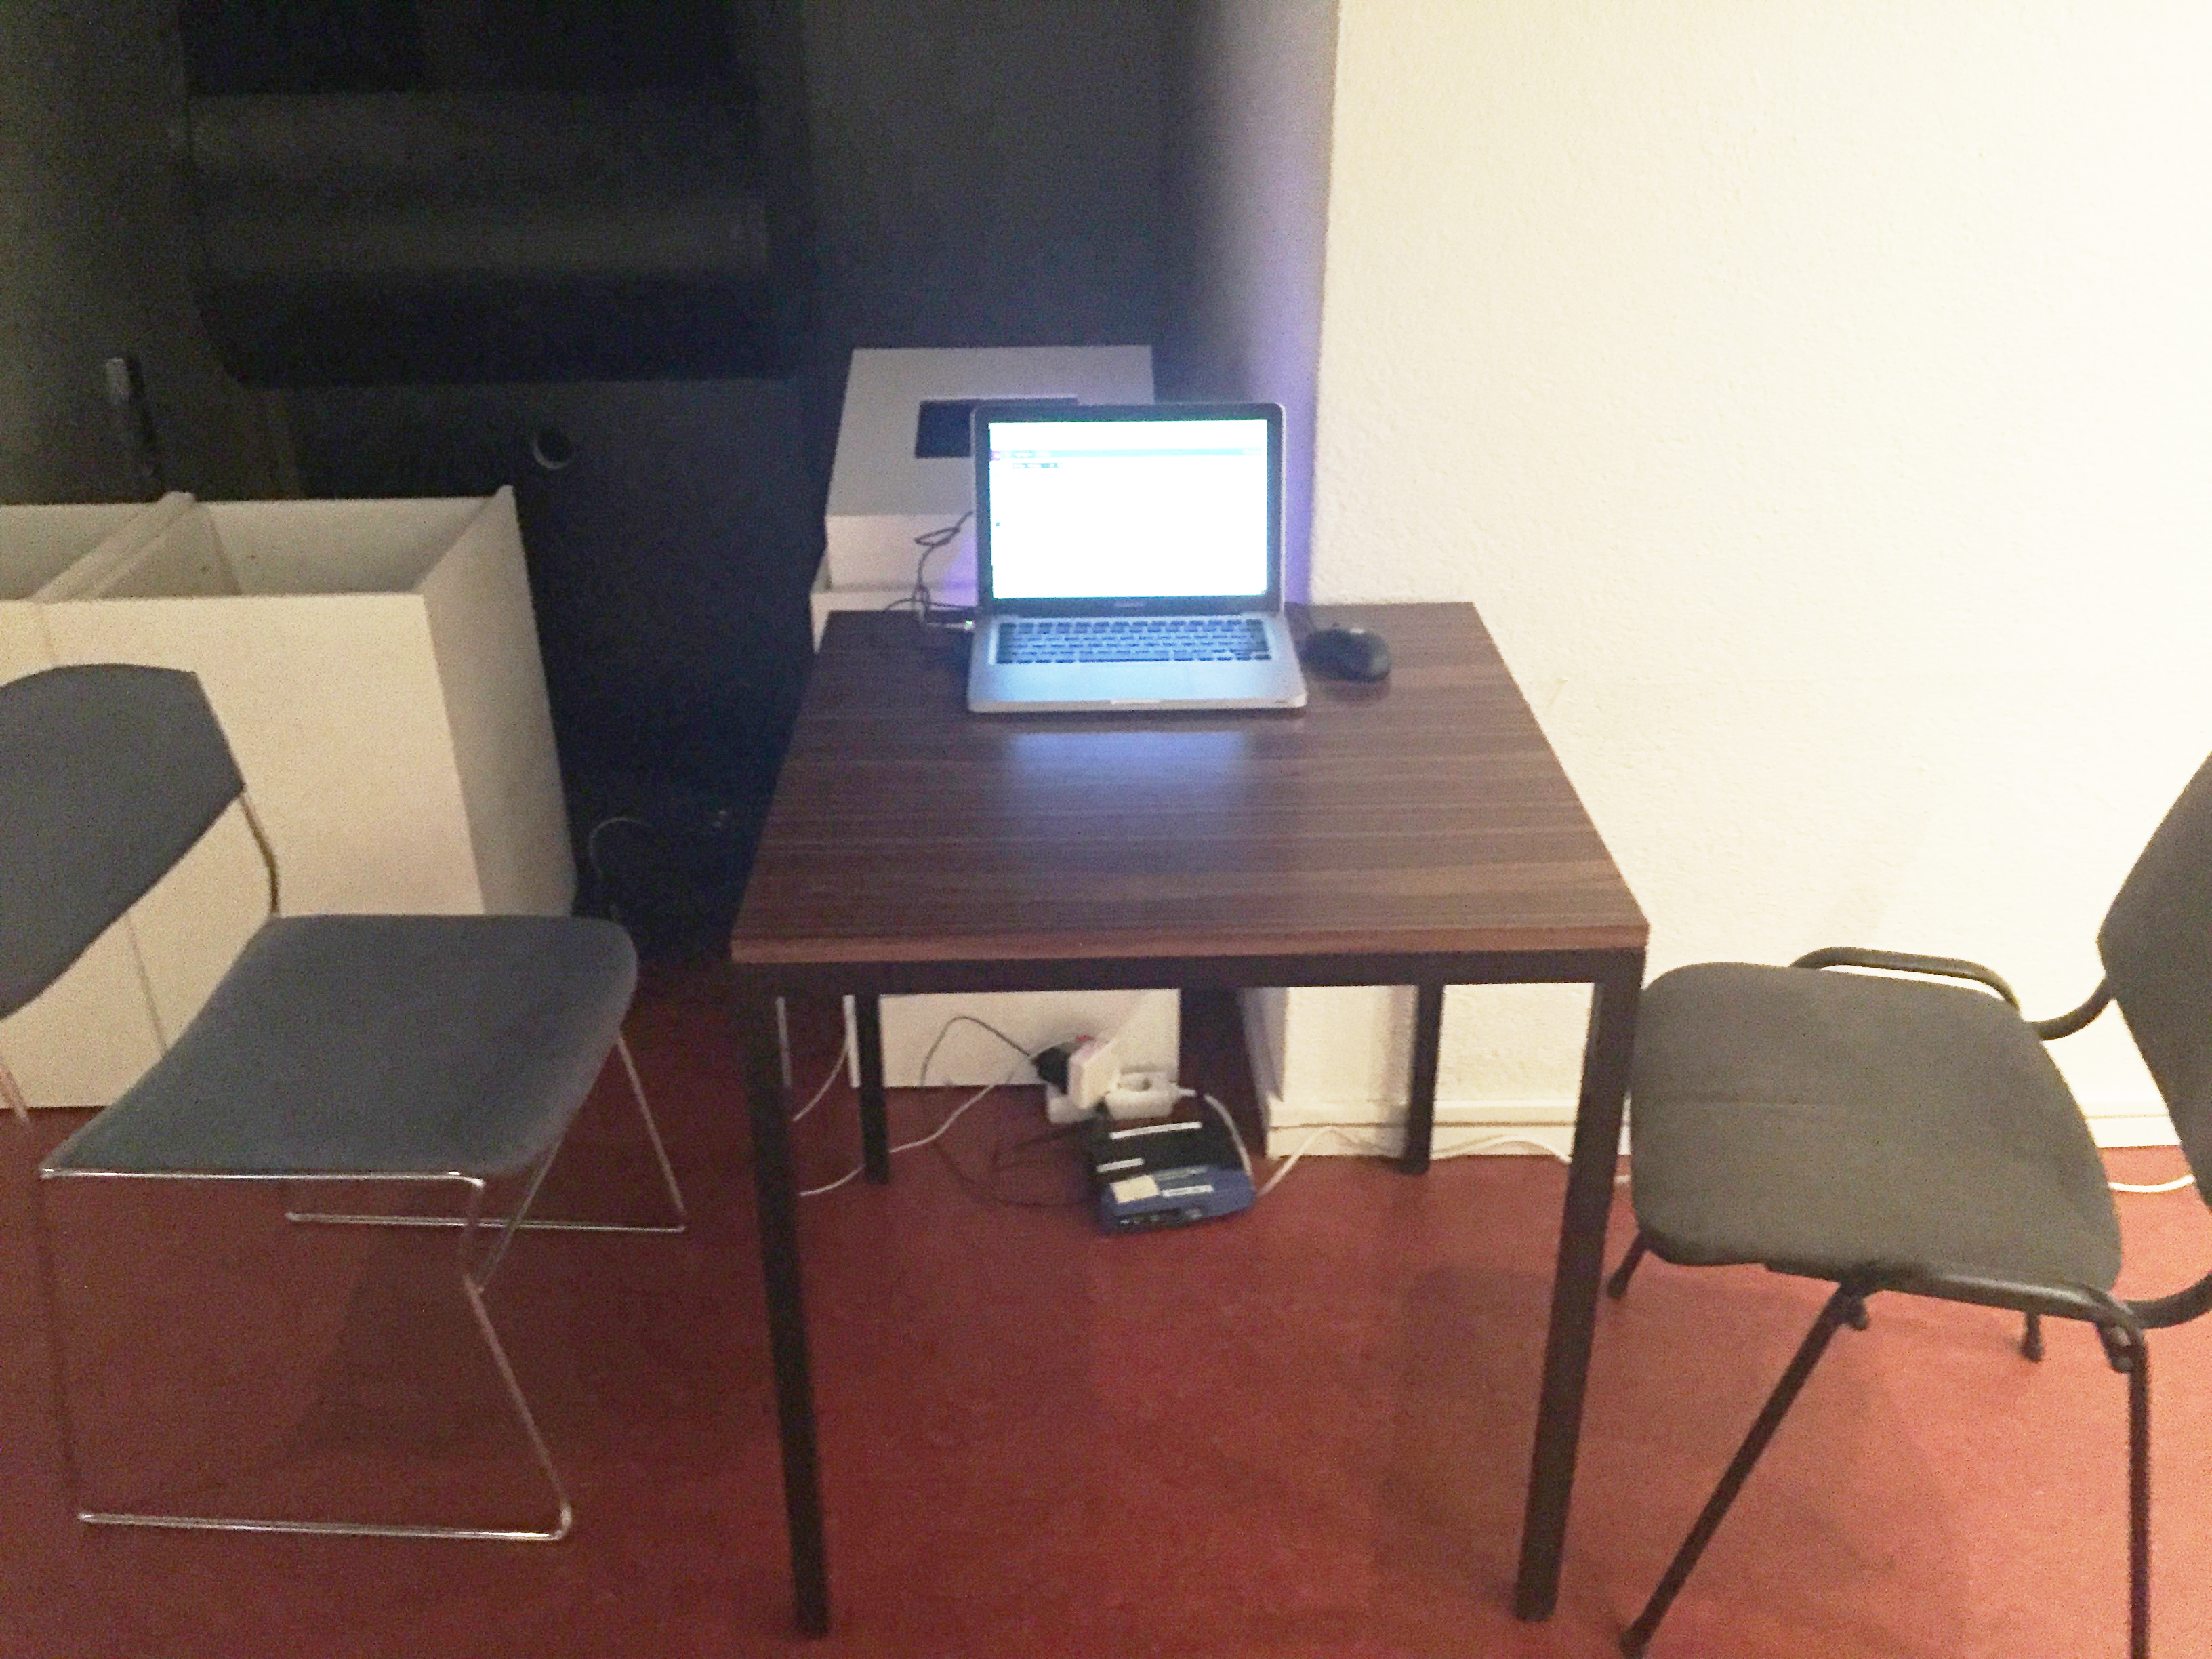
\includegraphics[width=.3\linewidth]{study/desktop_b.JPG}}\hfill
\subfloat[A projector augments a plinth with an artefact on it.\label{fig:example}]
  {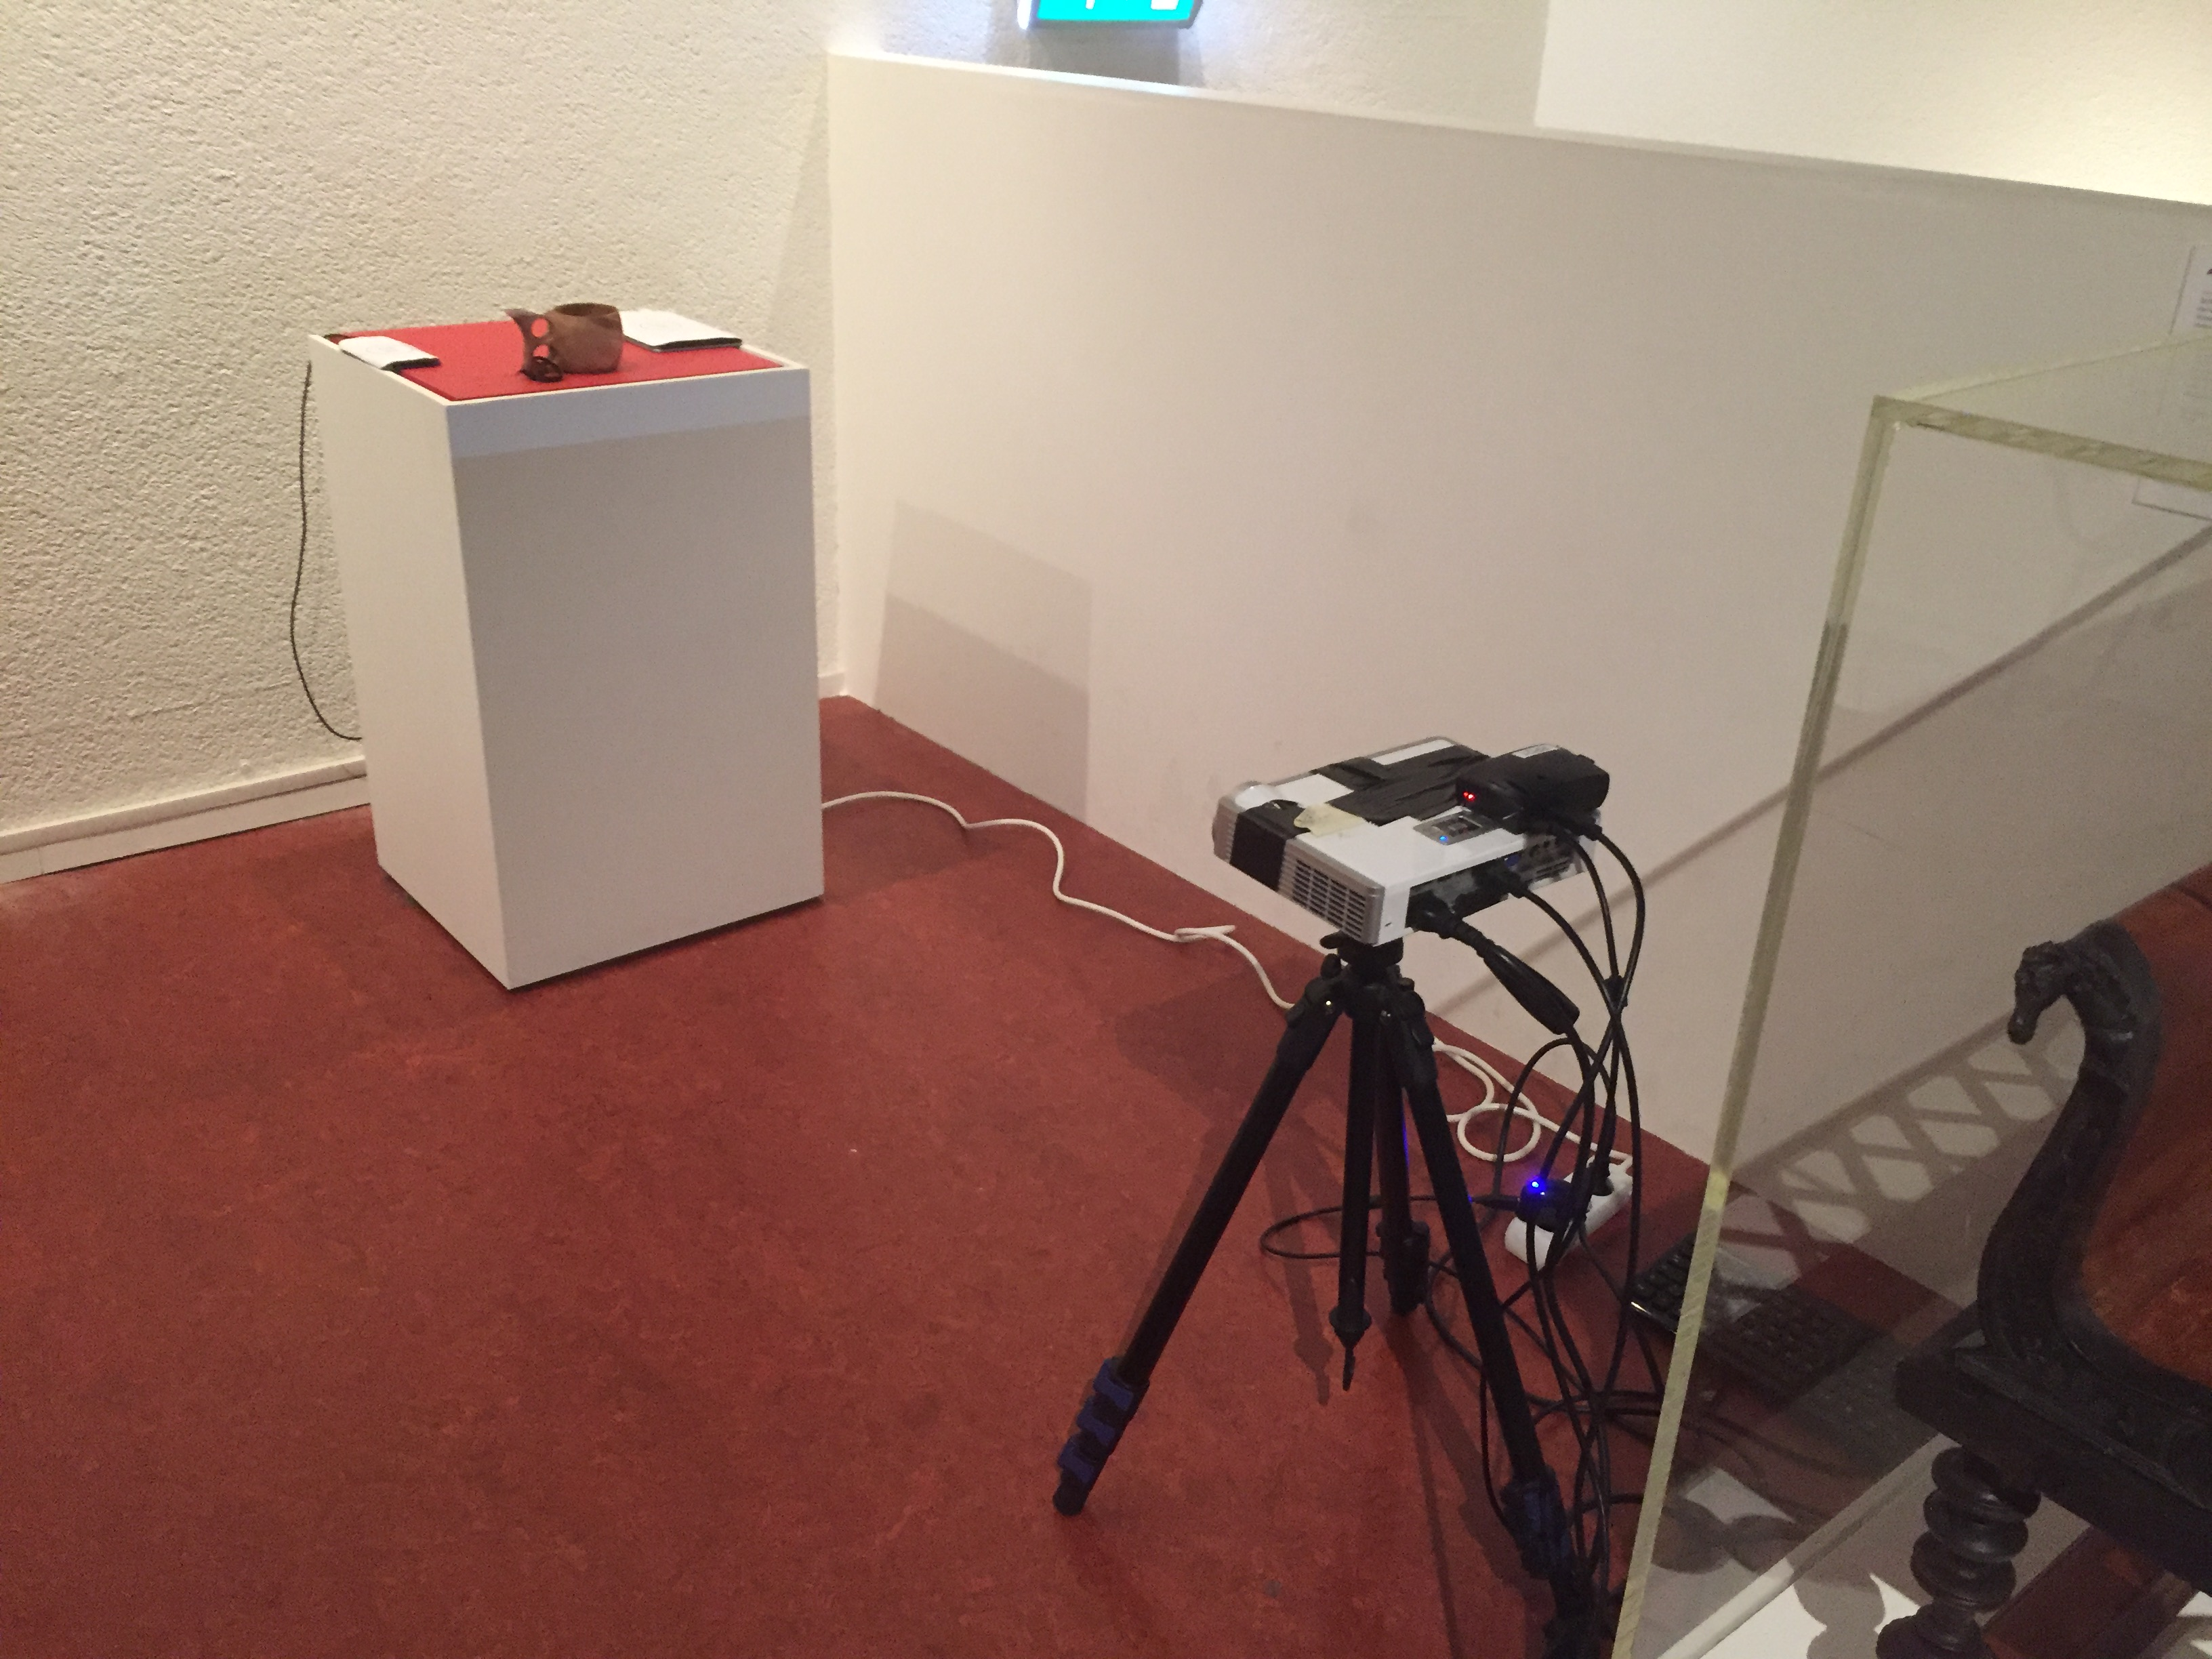
\includegraphics[width=.3\linewidth]{study/setup.JPG}}\hfill
\subfloat[The tangible cup and the two NFC-Reader\label{fig:kuksa}]
  {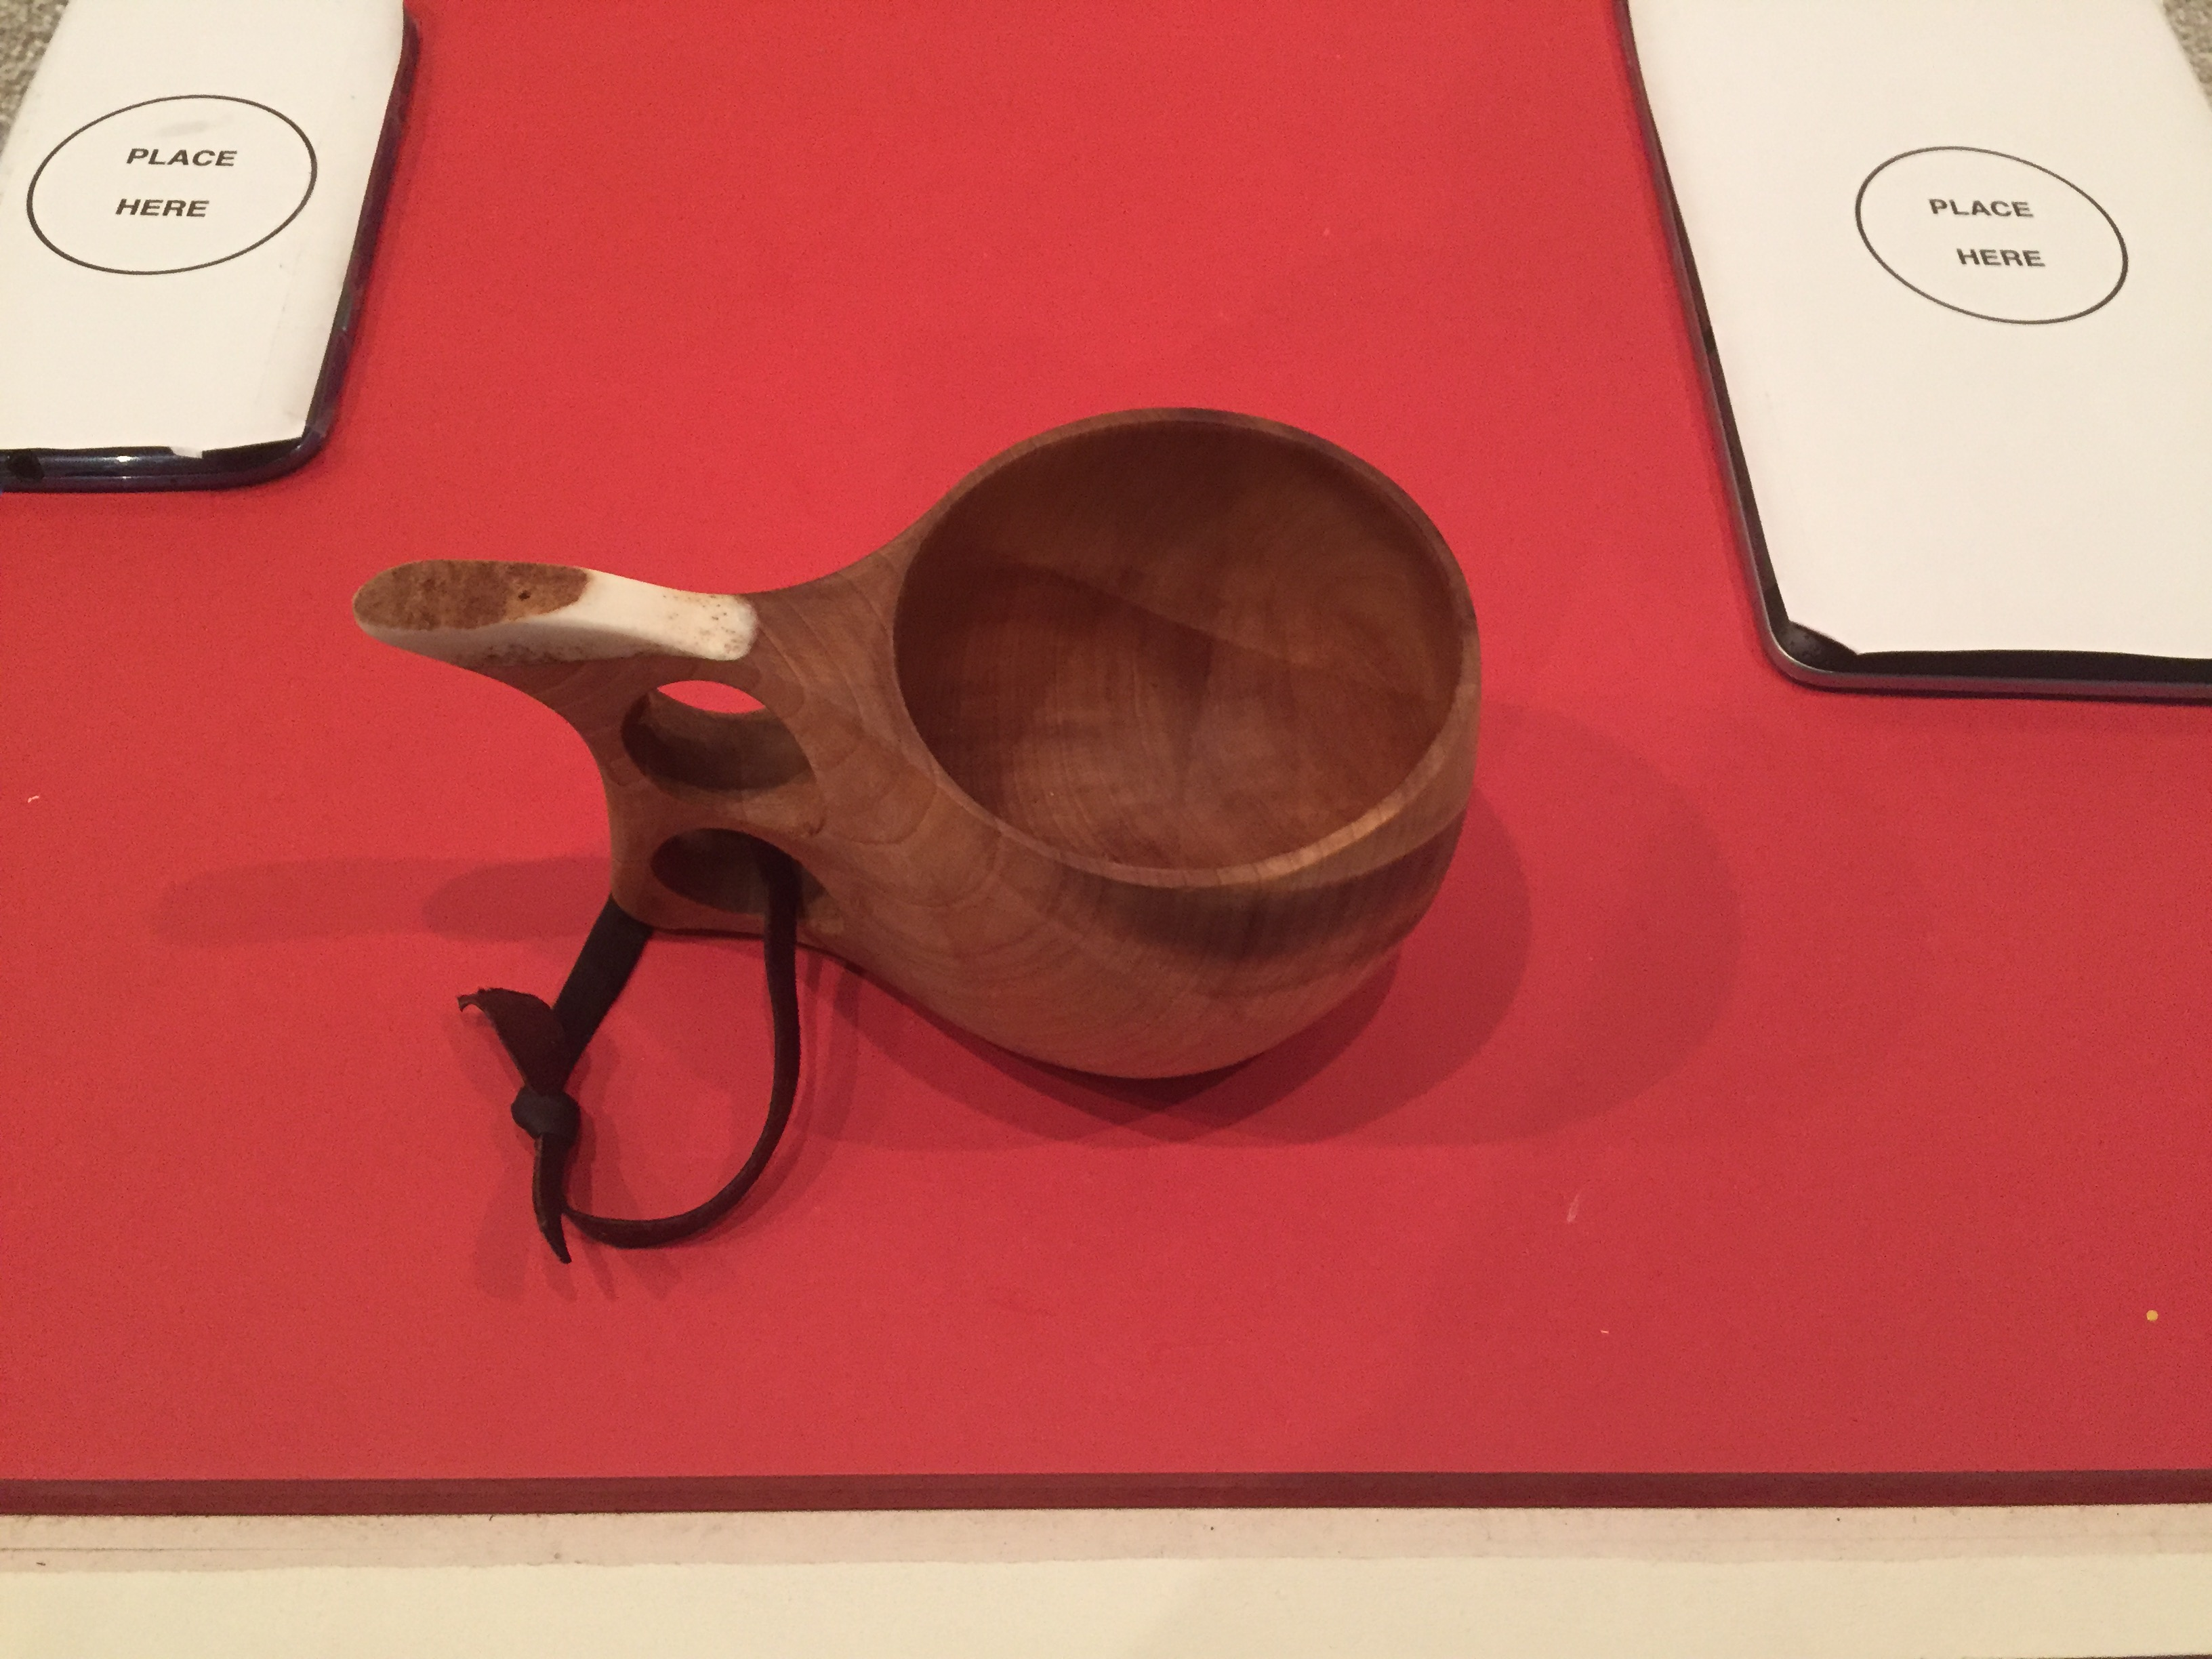
\includegraphics[width=.3\linewidth]{study/kuksa.JPG}}\hfill
\caption{The general setup of the study}
\end{figure}

For the study 5 participants (all) with an average age of 38 years (50+ highest, 22 lowest) and a different level of technical expertise were recruited. Every participant had to fill in a short questionnaire (see Appendix \ref{generalbackground}) about their general background which includes questions about their gender, age, profession and experience in designing interactive and non-interactive exhibitions (1 - No experience, 5 - A lot experience). The general background questionnaire showed that the participants were working in a variety of different professions. There was a media manager who is responsible for the collection of media and information for exhibitions in her museum as well as a student of museology, a filmmaker who develops interactive systems for a living museum, a museum professional/historian and a phd student of museology.  Therefore, the experience in creating exhibitions was very low, only one participant had a score of 4 in creating exhibitions at all. In total the participants had a score of 2 in experience on creating exhibitions and a score of 1 in experience on creating interactive installations. Only one participant had some experience with creating interactive exhibitions. The participants where not required to have any technical expertise and were selected randomly. Three of five participants were actually working in a museum, one of them wants to work in the museums field after her study and one is supporting curators creating installations once in a while. The participants did not get any reward for participating at the study.

The study-environment was set up in one exhibition room of the museum. On one side there was a table with a desktop computer which represented the participants' office. There the participants had to create and compose content and configure behavior rules for their interactive installation. Furthermore, a server instance of the meSchup platform was running on the desktop computer. On the opposite side a projector connected to a RaspberryPi was set up to be used as displaying component for the interactive installation. In front of the projector there was a one meter high wooden box on which two NFC-Readers where placed as well as a replica of a traditional Finnish drinking cup "Kuksa" which should be used as tangible object to execute the interaction. The NFC-Readers where two Android devices which where hidden by using paper to hide the technology from the participant. On the bottom of the drinking cup a NFC-Tag was posted. Besides, there was set up a second RaspberryPi connected to a second projector as a demo installation. This setup was used to demonstrate the participants how the system works and gave them one example of what can be done. Therefore, an interactive installation in form of an info point was realized. First a big info sign and the text "Come closer to get more information" was shown. If a participant comes closer the content changes and shows directional instructions. Furthermore, a Wifi Access Point was set up to create a wireless local area network to which all devices where connected. All RaspberryPies, the distance sensor and the two Android devices which where used as NFC-Readers where configured within the meSchup platform in advance. One assumption was that the participants would not take part in setting up the technical part in their working environment so they do not have to in the study as well. Additionally, two behavior rules where implemented. One for the Distance Sensor used in the demo and one for the task the participants should handle. A further assumption was that cultural heritage professional will not be able to code the behavior rules on their own, so these templates which they should configure were provided. Furthermore, an iPad Air was prepared as mobile device which should be used to adapt content on-site.

\subsection{Procedure and Tasks}

\begin{figure}
\subfloat[Participant composes content on desktop computer\label{fig:user}]
  {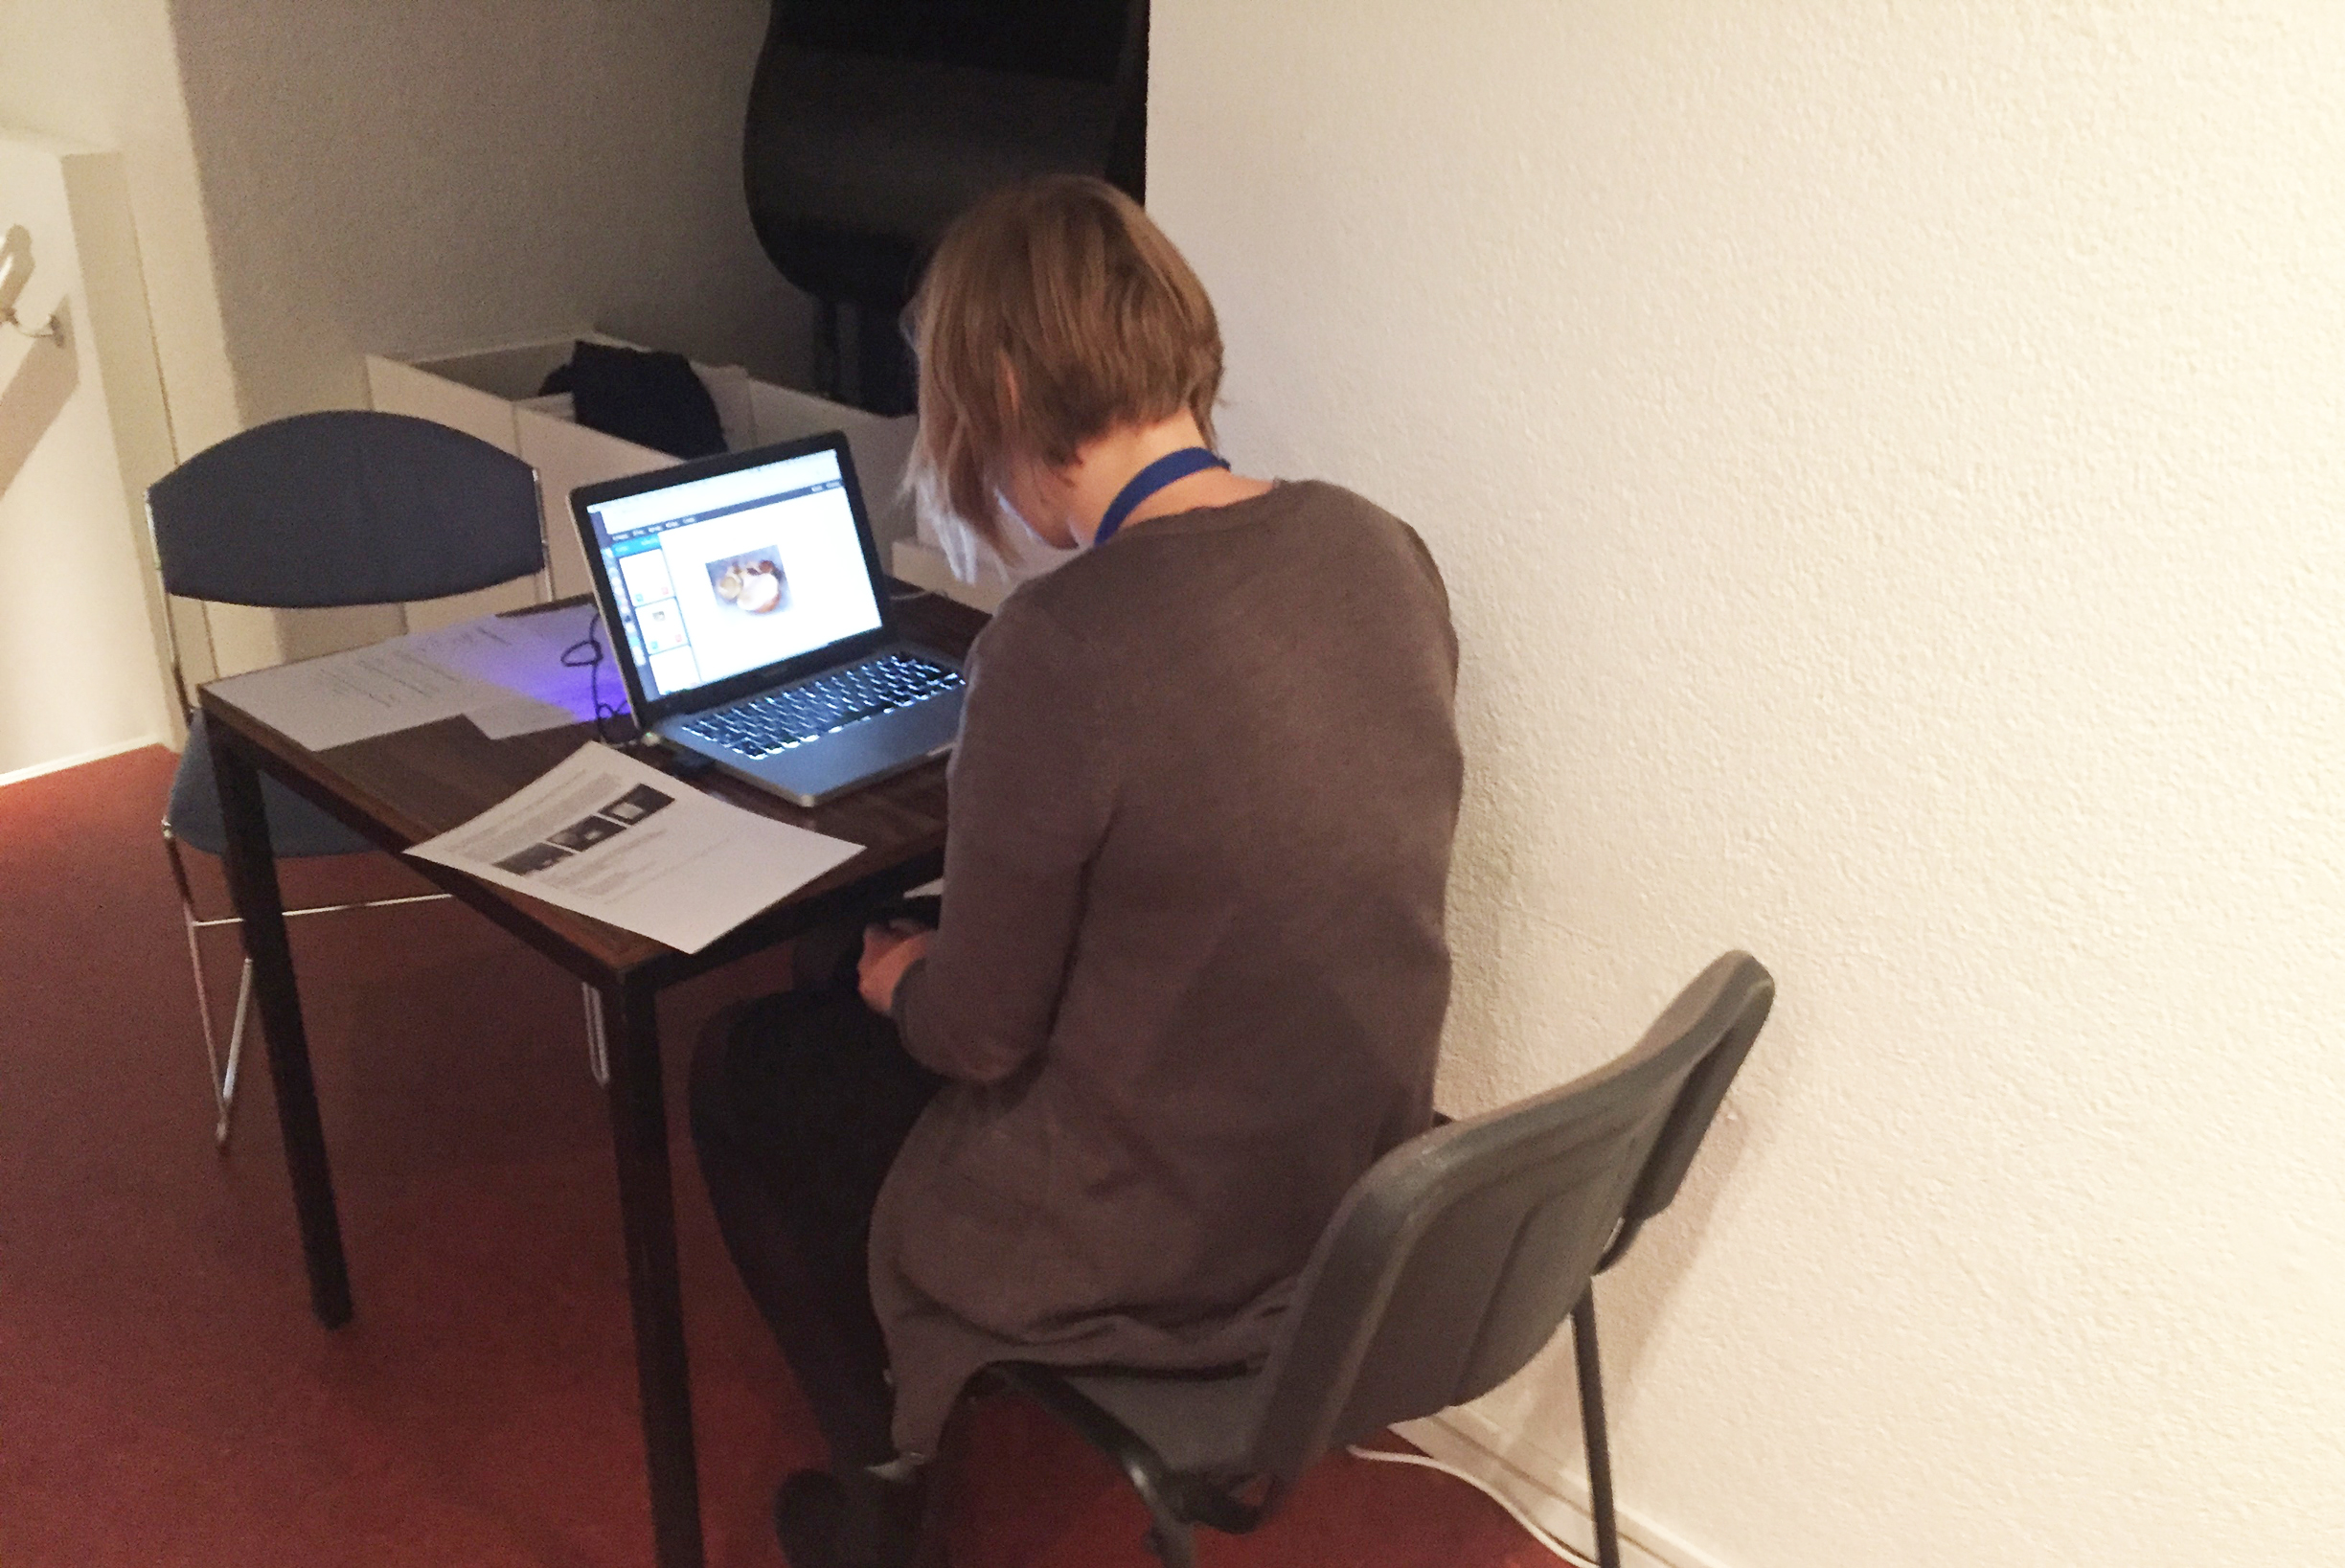
\includegraphics[width=.3\linewidth]{study/user.JPG}}\hfill
\subfloat[Example content of a participant\label{fig:example}]
  {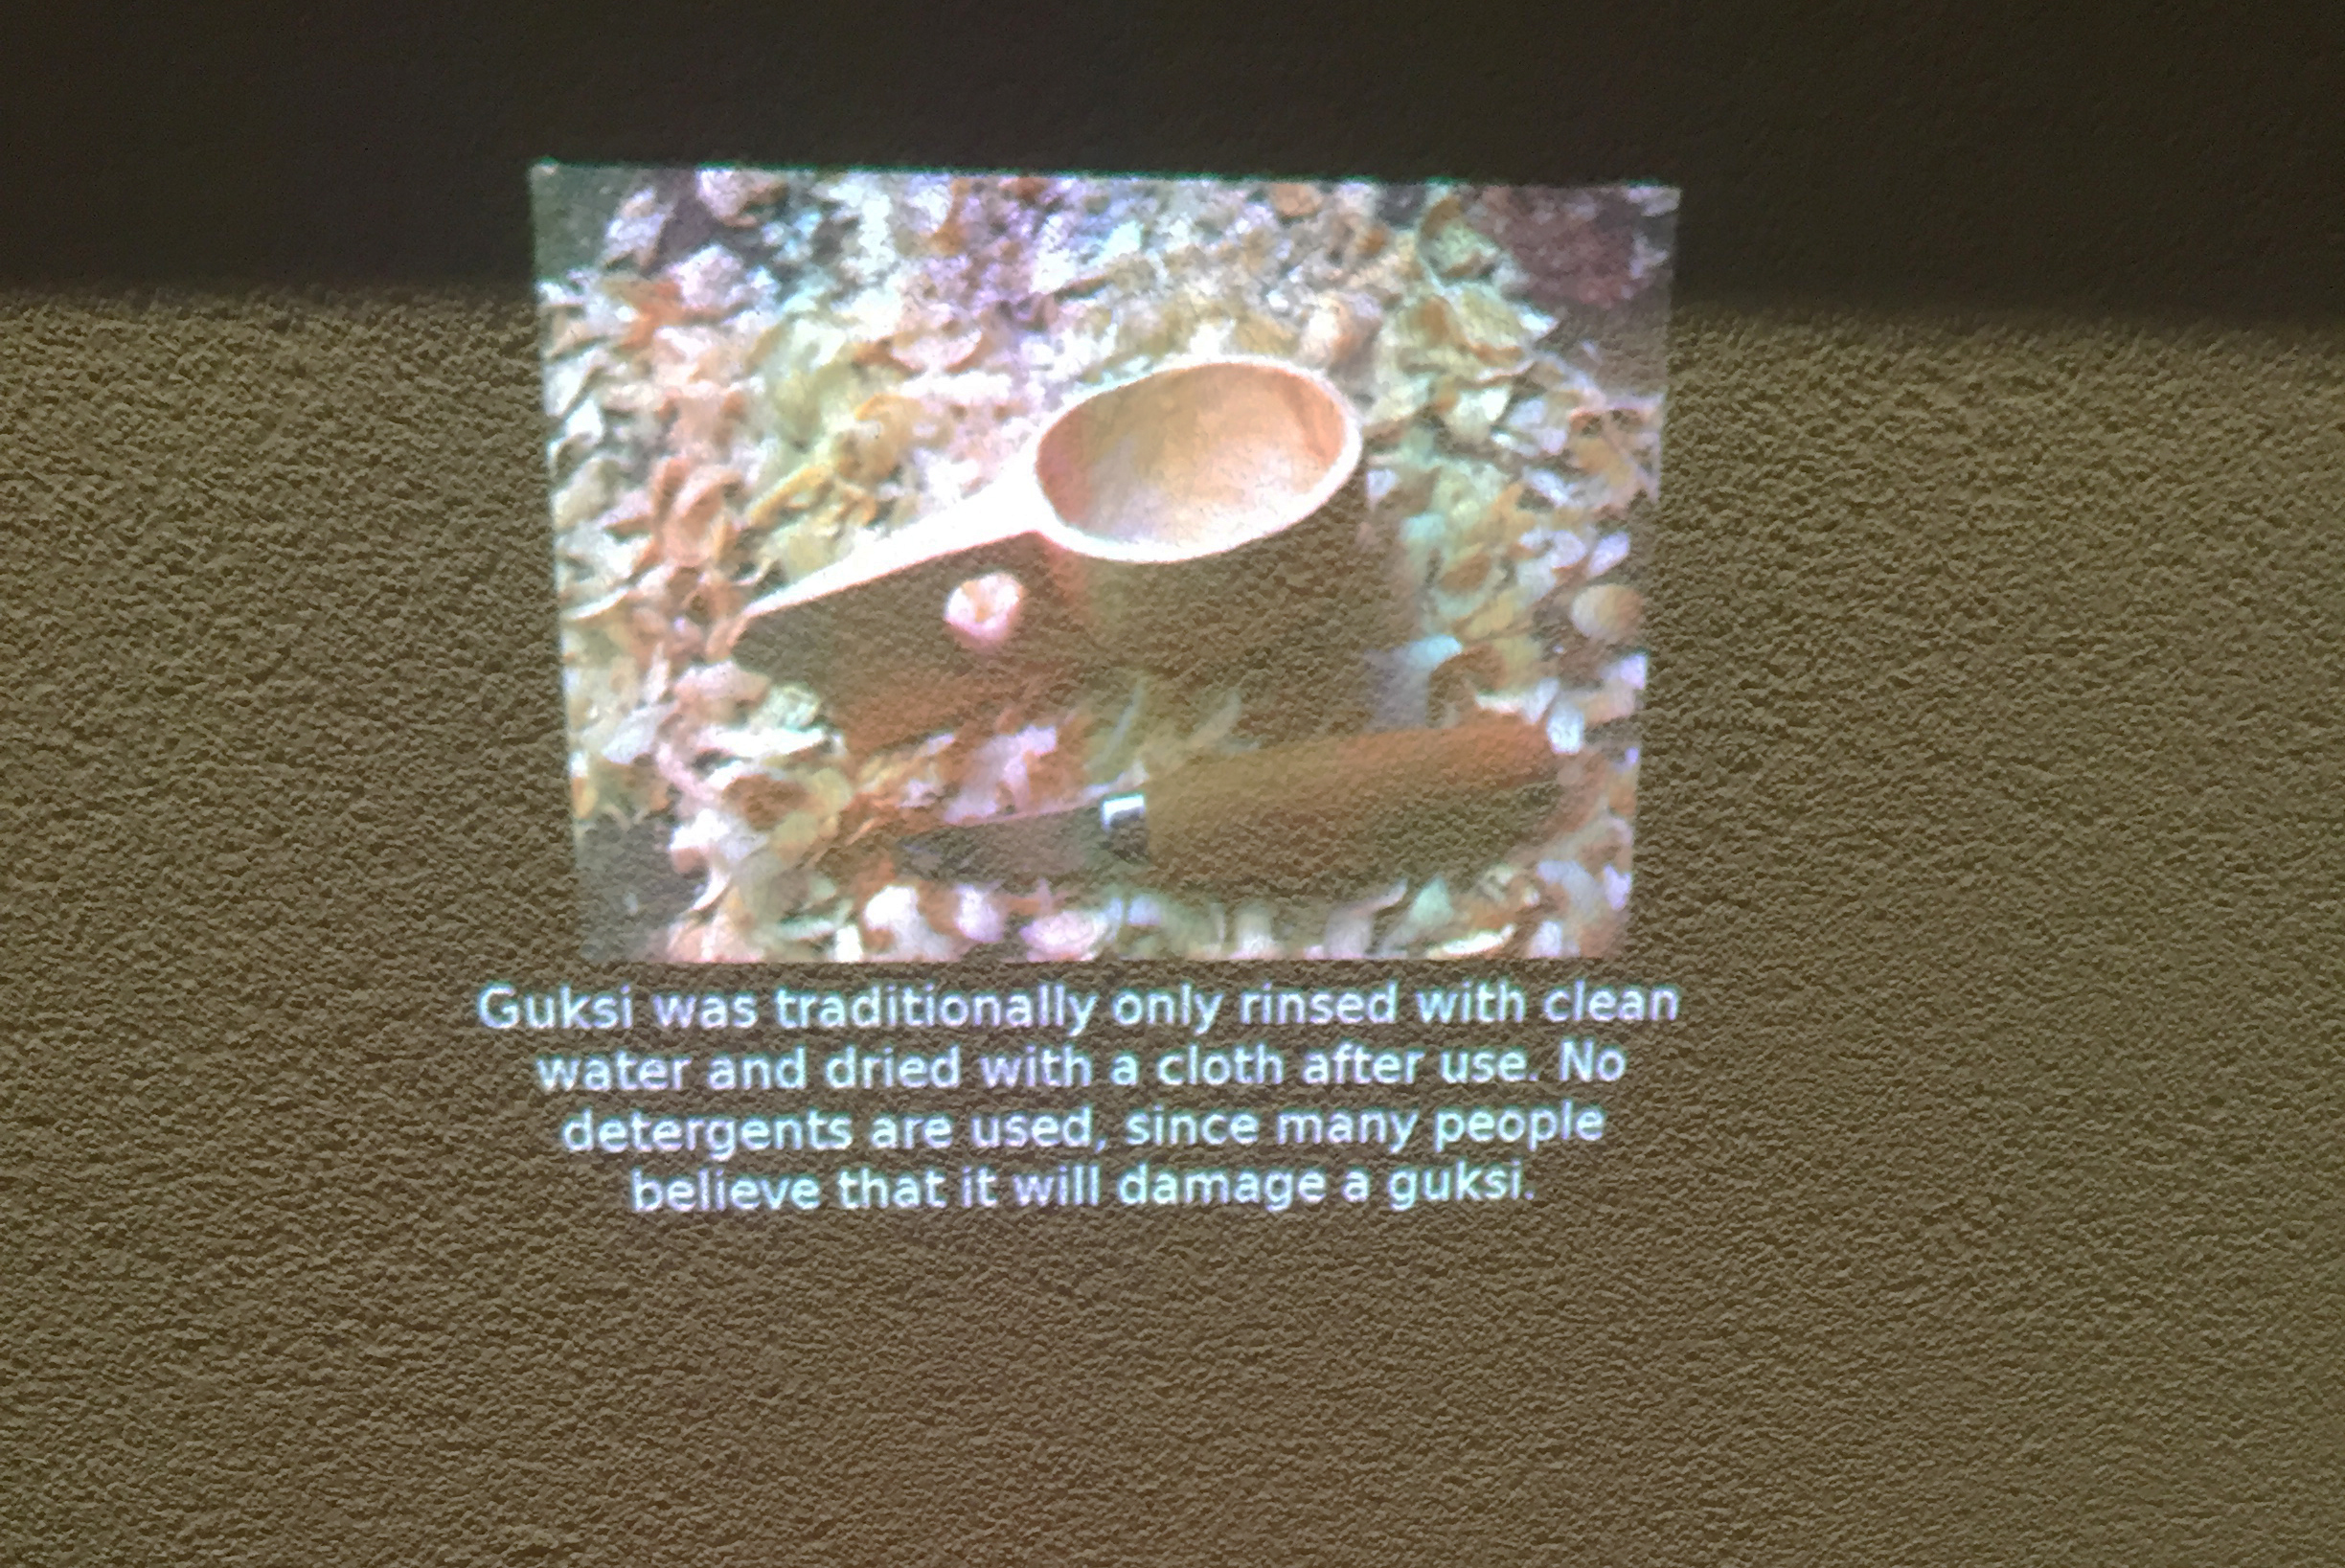
\includegraphics[width=.3\linewidth]{study/example1_b.JPG}}\hfill
  \subfloat[Cup augmented with projected text\label{fig:mo_me}]
  {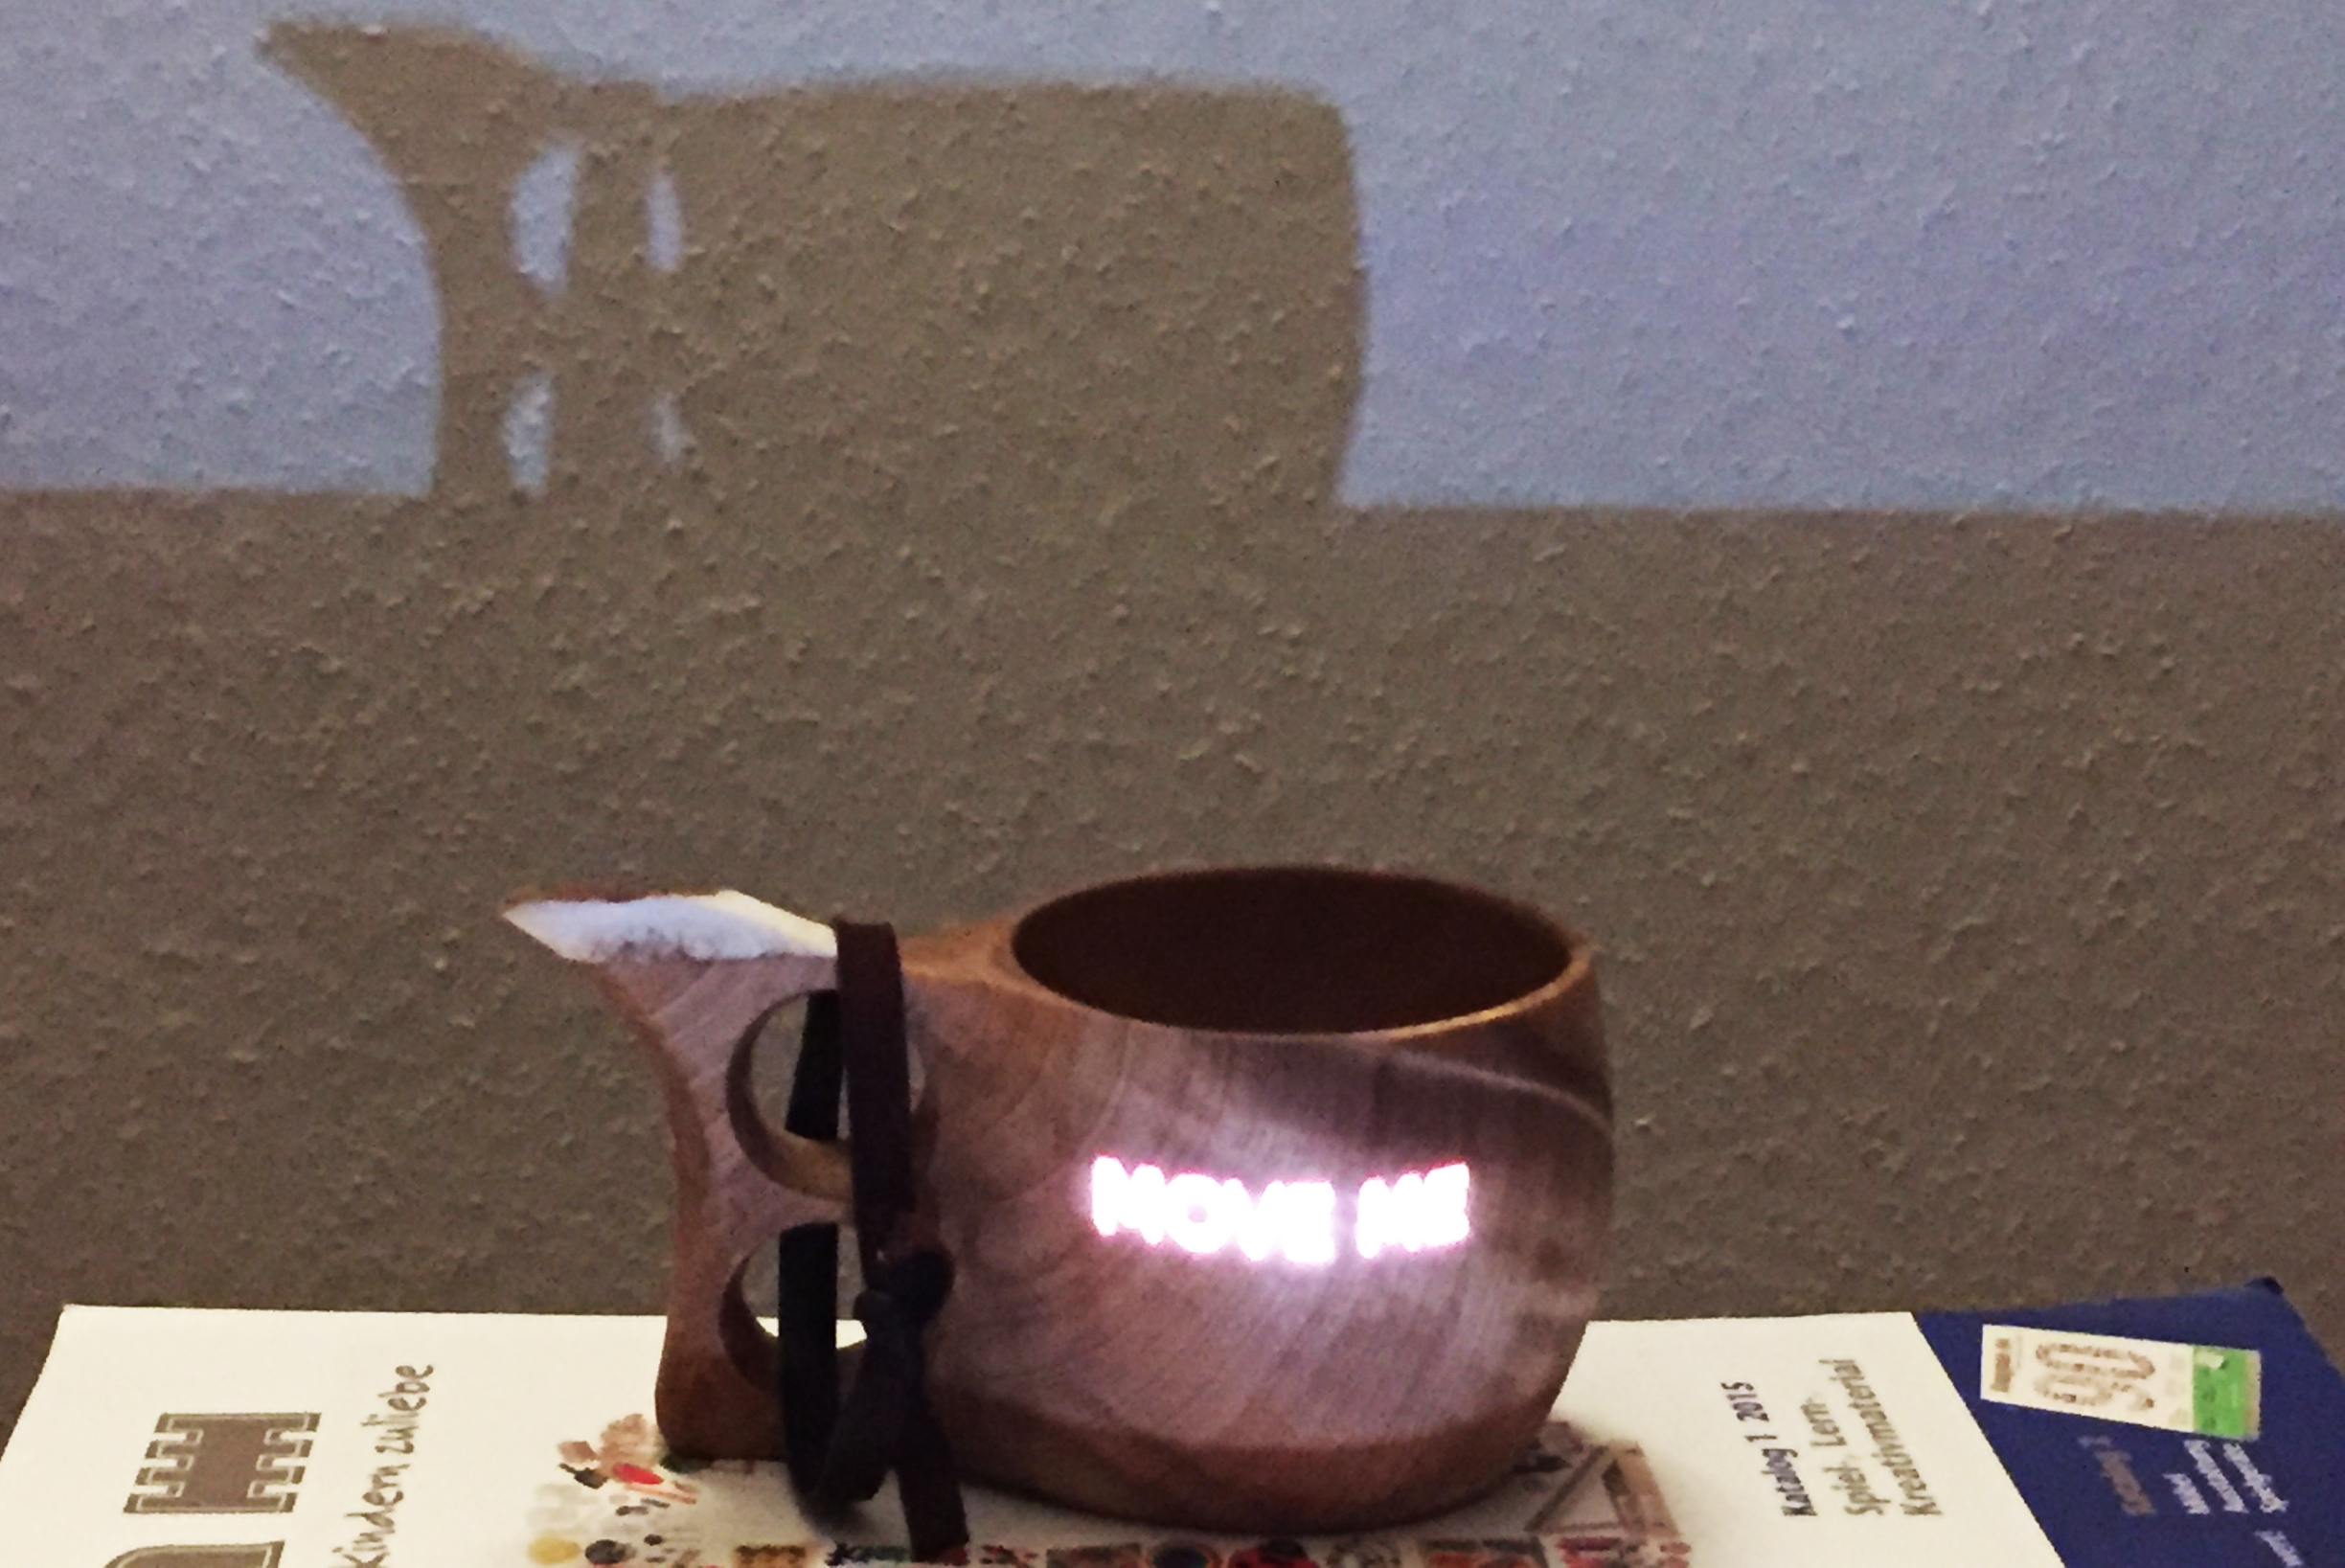
\includegraphics[width=.3\linewidth]{study/mo_me.JPG}}\hfill
\caption{Participant during the study}
\end{figure}

Every participant was welcomed at the reception of the museum and accompanied to the study set up. There the participant needed to sign a consent form (see Appendix \ref{consentform}) and fill out a short questionnaire about their general background. Afterwards they got a detailed introduction into the system and a demonstration by using the demo project. Then the participants where introduced into the task they should solve. Therefore, a short story was told. The participant should imagine being a curator who wants to create an interactive exhibition about the traditional Finnish drinking cup "Kuksa". The participant should create three slides, create a behavior rule by using a template and configure it using the VEII Rule Editor. Last they should test the created exhibition by moving the cup. The task was divided into the following steps:

\textbf{Step 1: Content creation}
\newline
The participant should create three slides with different content on the desktop computer. With the first slide the Finnish drinking cup should be augmented with a projected text like "Move Me".

\textbf{Step 2: Creating interactivity} 
\newline
The participant should use a template to create a rule which provides the NFC functionality. There the participant had to choose the two NFC-Readers as well as the slides which should be displayed.

\textbf{Step 3: Deploy Content} 
\newline
The participant should deploy the created content on the display device by using either the desktop computer or the mobile device.

\textbf{Step 4: Adapt content on-site} 
\newline
The participant should visit the installation with a mobile device and adapt content according to the environment.

\textbf{Step 5. Switch to deployment mode:} 
\newline
The participant should use the mobile device to switch the installation from the "Live-Edit" mode to the "Deployment" mode.

\textbf{Step 6: Test the interactivity} 
\newline
The participant should move the Finnish drinking cup and place it on the different NFC-Reader to test the interactivity.

The participants were allowed to ask questions during the whole study. After finishing the task, every participant had to answer a System Usability Scale (SUS) questionnaire with 10 questions. Afterwards each participant took place in a semi-structured interview which lasted about 15 to 30 minutes. The questionnaire is shown in Appendix\ref{prestudy}. On average, the total duration of a study with one participant lasted 45-60 minutes.

\subsection{Study results and discussion}
In this section the observations about participants' creation strategies as well as the results of the System Usability Scale (SUS) questionnaire, the participants qualitative feedback is discussed.

\subsubsection{Creation strategies}
During the study all participants created their own interactive installations with digital content using NFC technology and a tangible cup as trigger. The average completion time was 22 (12 lowest, 43 highest) minutes. An observation was that the participants had different creation strategies. P1 started designing her exhibition on a piece of paper and tried to rebuild it within the VEII Slide Editor. P3 and P5 where more respectful towards the system and thus slowly started to gain an overview of the system before actually creating content. In the opposite P2 and P4 where very fast in creating the needed slides. P1 said, \textit{"It's very easy to use, I'm used to this kind of system"} and P2 thought it was \textit{"very easy and super handy"}. After creating and composing the content on different slides the participants added behavior rules. Firstly it was hard for the participants to understand what "rule" actually means. P1 mentioned: \textit{"My first impression was, what kind of rules?"}. After explaining it in detail and calling the rules "behavior rules" the participants got used to it. P1 and P5 exceeded the task and were trying to create way more complex interactivity than expected which was not possible because only the specific template for the planned interactivity were provided. On the one hand P1 and P5 discovered a bottleneck of the current system. If there is no suitable template for the desired interactivity, creators have to call an expert who implements a new template. On the other hand it shows how the system promotes playful experimentation. P1 and P5 got excited using the system and therefore wanted to create advanced interactivity in the same way they would do it in their professional environment.  
After creating the behavior rules, the participants went on deploying the project on the display device and using the mobile device to adapt content on-site. P4 mentioned: \textit{"The fast change between desktop and mobile is very good and practical"}. All participants modified the created content to match the position of the wooden box. Furthermore, the participants did not know where the cup is standing while they created the content on the desktop computer so they needed to position the "Move me" text on to the cup using the mobile device. P5 added: \textit{"I really liked it that I could augment the cup, I did not think about using projectors this way by now"}. Next the participants had to set the project to deployment mode. Some participants had some issues with the different modes for example P2 said, \textit{"I was a bit confused by the live-edit and deployment-mode. You have to get used to it, but it makes sense to work in a live- and an edit-mode"}. Last the participants tested their installation by moving the cup to the different NFC-Readers.

\subsubsection{Working with the system}
The participants found the VEII toolkit was intuitive to use and easy to learn which is reflected by the average score of 4.0 (SD = 0, 0.0 - lowest, 4.0 - highest) of the question \textit{"I would imagine that most people would learn to use this system very quickly"} in the SUS. One assumption was that the system is very usable for users who do not have any technical background. This is confirmed by the average score of 3.8 (SD = 0.4) of the question \textit{"I think that I would need the support of technical person to be able to use this system"}. Despite the positive review on the ease of use of the system, participants felt less confident while creating an interactive installation. The question \textit{"I felt very confident using the system"} only got an average score of 3.0 (SD = 0.63). A reason for this could be the short usage time. Participants where using the system for the first time and only about 30 minutes. The VEII toolkit ended up with a total score of 89.0 in the SUS. In Figure~\ref{fig:studyresult2} the results of the SUS are shown ordered by participant. Every question got a score above the standard average score of 68 which is the threshold of a usable system.
\newline

\begin{figure}
  \begin{center}
    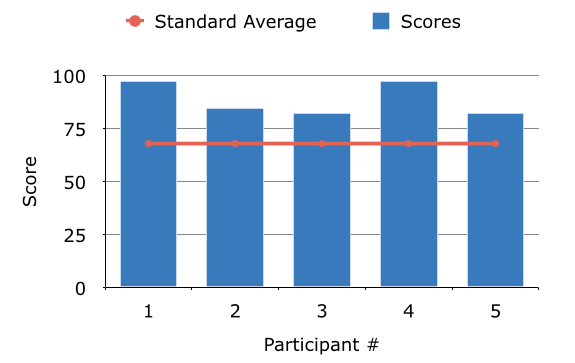
\includegraphics[width=.8\textwidth]{study/study2.png}
    \caption{The results of the SUS questionnaire by participants}
    \label{fig:studyresult2}
  \end{center}
\end{figure}

\textbf{Working with the VEII Slide Editor}
\newline
The participants where fast in learning how to use the VEII Slide Editor and called it \textit{"very easy to use"} (P4). Some of the participants where learning the system faster because of structural similarities to existing software. P2 mentioned: \textit{"Parts of the system reminded me a bit of how you edit information in Wordpress"}. But also participants without any technical background got used to the VEII Slide Editor fast. P5 said, \textit{"First I was not sure how to create content and how to use the slides, but after a few minutes it was easy"}. In opposite to the first study the participants in Amsterdam where missing some additional features within the editor. They were asking for a possibility to add basic shapes like rectangles, circles or arrows to highlight specific elements of the view. Therefore, P1 said, \textit{"The possibilities for designing slides seemed a bit limited"}. Furthermore, P1, P2 and P4 wished for a method to provide slide templates. A slide template would contain multiple fixed empty content entities which then can be replaced by the creator. So creators can secure that all of the slides will be structured the same way and do not have to position the elements for each slide over and over again. P2 mentioned: \textit{"It would be nice to have a template which already contains positioned images and texts"}. Additionally, P2 suggested adding vertical and horizontal anchors to improve the alignment of content entities among themselves.
\newline

\textbf{Working with the VEII Rule Editor}
\newline
As already mentioned, the participants had some issues with the term "rule" itself. It was not entirely clear what is meant and what is regulated by those rules. Furthermore, the term "rule" cannot directly be connected to the interactive behavior which should result from creating rules in the VEII toolkit, therefore it is understandable that the participants were confused. Thus, it was easy for all participants to add a rule by using a template and then configure it according to the task. P5 said:{"I really liked the configuration of the behavior. Just choosing the right device or slide was simple"}. P4 did not remember in which order she created the slides and therefore could not select the specific slide during the rule configuration without getting back to the VEII Slide Editor. Afterwards P4 suggested selecting the slides in the rule editor by a predefined name and not by a number. An alternative approach would be to show a slide preview within the rule editor. P1 suggested a new feature which enables to switch slides automatically after a specific time period. Furthermore, P1 proposed to implement the creation of interactivity in a way which is more similar to creating animation in Microsoft Powerpoint. Therefore, using multiple states of content entities and define the transition between them by choosing from a predefined list of animations. All in all the participants had a positive impression of the VEII Rule Editor and the rule templates. P1 noted: \textit{"I would need to get used to the rules, but I could imagine using them to define behavior"}.
\newline

\textbf{On-site editing}
\newline
The participants were impressed of the possibility to compose and adapt content using the mobile device and getting immediate feedback from the system. P4 said, \textit{"Seeing how the adaptation I did on the iPad directly on the projection surface was great. It is really useful"}. P2 added, \textit{"I could easily take my iPad and go on site and see how it looks and then adjust content"}. P1 noted: \textit{"It is easy to edit on the spot especially wrong positioned content or spelling mistakes"}. However, all participants met with a difficulty which affects the mobile device and rich text. All text within the VEII Slide Editor is written and modified in a rich text editor. Within this rich text editor it is very difficult to change the font size of the selected text. P2 said, \textit{"Unfortunately I could not change the font size using the iPad"}. P1 added: \textit{"There should be provided an improved way to modify the font size on the iPad"} and P2 mentioned: \textit{"It was really hard to change the font size on the mobile device"}. Furthermore, P2 was a bit worried of older curators and the VEII toolkit. P2 said, \textit{"All the curators are men who are like 60, so for them it would be a little bit harder to start using it but it is so simple, I think they will not have lots of problems with it either"}. Despite of the adaptation of the font size, the participants where excited about the on-site editing approach.

\textbf{Feedback}
\newline
Furthermore, the participants where asked if and how they would use the VEII toolkit in their professional environment. P2 took up the approach of using a tangible object for the interactivity. P2 said, \textit{"If I would make an exhibition and I would have something interactive like a 3D scan of an actual object, then it would be really great to have someone interact with the object and then get the according information."}. P3 however thought about deploying the system in a living museum. P3 wanted to create multiple interactive exhibitions within the living museum and combining them with the living exhibits. P3 said, \textit{"Creating interactivity not only by using objects but by using the exhibits themselves would be a great idea"}. P4 mentioned: \textit{"The system is a great solution for especially highlight one or two items in an exhibition which is overall more traditional"}. Therefore, P4 thought about enhancing traditional exhibitions by adding interactive components. P5 was particularly excited about the possibility to change content fast. P5 thought about changing exhibition content on a daily basis to adapt the information according to requirements of the visiting group of people. For example P5 mentioned adapting the content for a group of children on the first day and on the next day receiving a group of older guests and show different content. This kind of changing content or the presentation of content on a daily basis is not possible the way P5 is creating exhibitions by now. Furthermore, P5 was thinking about connecting the VEII Slide Editor to the internet. In particular P5 imagined school children to create their own interactive exhibition at home one day before they are visiting the museum. Curators would now be able to deploy those exhibitions in different places of their museum, so children could visit their own exhibitions the next day. P5 added: \textit{"School kids would remember the things they need to present better because they have to prepare it in a new way and further have the possibility to present it to their classmates in a real museum. I imagine them saying: 'Hey, look what I did!' "}. All in all the participants where excited about the possibilities of the system especially because it is providing flexibility for the location and the content of an exhibition. P4 mentioned: \textit{"As far as I know such a system is not available yet, a system that uses the more advanced sensors and that is so easy to adapt and to use and configure it by yourself"}.

\iffalse
P1: 
- "It's very easy to use, I'm used to this kind of system, like also in website design e.g Wix.com"
- not lot of options
- put in templates
- introduction
- easy to edit on the spot like typo
- seems really connected 
- timebased slide change

rules
- My first impression was, what kind of rules?

- add shapes (lines, dots, circles, arrows, ...) 
- powerpoint feature like fade should result into a rule

P2:
- "reminds a bit of how you edit information in wordpress"
- "very easy and super handy"
- "I could easily take my iPad and go on site and see how it looks and then adjust content"

- "It would be nice to have a template which already contains positioned images and texts."
- creating anchors for images.

- "I was a bit confused by the live-edit and deployment-mode. You have to get used to it, but it makes sense to work in a live and a edit mode".

- "If I would make a exhibition and I would have something interactive like 3D scan of an actual object then it would be really great to have someone interact with the object and then have the according information."

- "All the curators are men who are like 60, so for them it would be a little bit harder to start using it but it is so simple I think they will not have lots of problems with it either"

P4: 
- "Very easy to use"
- "The biggest thing I would add, is if you choose the slide in the rule to see which slide is which"
- font-size
- "The fast change between desktop and mobile is very good and practical"
- slide templates 
- great solution for especially making one or two item in an exhibition which is overall more traditional
- As far as I know such a system is not available yet, a system that uses the more advanced sensors and that is so easy to adapt and to use and configure it by yourself.

P5:
- see paper

\fi 

\section{Summary}
The VEII toolkit was evaluated within two studies. The first study was a pre study to test the usability of the toolkit with focus on the qualitative feedback from the participants. With a score of 82.5 the toolkit reached a high usability and especially stands out in its simplicity for new users to learn to use the system. The qualitative feedback nevertheless opened up some consistency gaps within the system which could be closed afterwards but also showed new perspectives and new usage scenarios like using VEII to create appealing exhibitions on fairs.
The second study was focused on the qualitative feedback of the cultural heritage professionals, furthermore the usability was tested as well. With a score of 89.0 in the SUS the improvements implemented (e.g. using tooltips to give more feedback to the user) after the first study took effect. The qualitative feedback of the cultural heritage professionals opened up new ways to look at the system. They put the emphasis on things that were not previously considered like the importance of aligning content or the different usage possibilities.